\documentclass[journal,twoside]{IEEEtran}

\usepackage[T1]{fontenc}
\usepackage[utf8]{inputenc}
\usepackage{amsmath,amssymb,amsfonts}
\usepackage{amsthm}
\usepackage{mathtools}
\usepackage{booktabs}
\usepackage{array}
\usepackage{multirow}
\usepackage{longtable}
\usepackage{xcolor}
\usepackage{graphicx}
\usepackage{tikz}
\usetikzlibrary{arrows.meta,positioning,fit,calc,shapes.geometric,backgrounds,patterns}
\usepackage{cite}
\usepackage{url}
\usepackage[hidelinks]{hyperref}
\usepackage[capitalise,nameinlink]{cleveref}
\usepackage{stfloats}
\newcolumntype{L}[1]{>{\raggedright\arraybackslash}p{#1}}

\theoremstyle{plain}
\newtheorem{theorem}{Theorem}
\newtheorem{proposition}{Proposition}
\newtheorem{lemma}{Lemma}
\newtheorem{corollary}{Corollary}
\theoremstyle{definition}
\newtheorem{definition}{Definition}
\newtheorem{axiom}{Axiom}
\renewcommand{\theaxiom}{A\arabic{axiom}}
\theoremstyle{remark}
\newtheorem{remark}{Remark}

\crefname{axiom}{Axiom}{Axioms}
\crefname{definition}{Definition}{Definitions}
\crefname{proposition}{Proposition}{Propositions}
\crefname{lemma}{Lemma}{Lemmas}
\crefname{corollary}{Corollary}{Corollaries}
\crefname{remark}{Remark}{Remarks}

\newcommand{\J}{\mathsf{J}}
\newcommand{\Ful}{\mathsf{Fulfilled}}
\newcommand{\Vio}{\mathsf{Violated}}
\newcommand{\Pen}{\mathsf{Pending}}
\newcommand{\Ind}{\mathsf{Indeterminate}}
\newcommand{\Def}{\mathsf{Def}}
\newcommand{\obs}{\delta}
\newcommand{\truth}{\tau}
\newcommand{\supp}{\operatorname{supp}}
\newcommand{\cov}{\operatorname{cov}}
\newcommand{\dm}{\operatorname{dm}}
\newcommand{\detd}{\operatorname{det}}
\newcommand{\arm}[1]{\textup{\textsc{#1}}}
\newcommand{\family}[1]{\texttt{#1}}

\makeatletter
\newcommand{\tabinput}[1]{\@@input #1.tex }
\makeatother

\hyphenation{chor-eo-graphy de-ter-min-able Red-ex}

\markboth{WeOps Research Working Paper WP-2026-DM-01, October 2026}%
{Celestin: Dependency--Mechanism Adequacy}

\begin{document}

\title{Dependency--Mechanism Adequacy: A Formal and Empirical Framework for Coordination Protocols in Autonomous Multi-Actor Systems}

\author{Wislet~J.~Celestin%
\thanks{W.~J.~Celestin is with WeOps Research. Working paper WP-2026-DM-01, October 2026. The executable models, benchmark outputs and independent arms are available at \url{https://github.com/Wescome/dmat}.}}

\maketitle

\begin{abstract}
Coordination protocols are usually judged by whether their executions conform to a specification. That is distinct from whether a protocol manages the dependency it exists for, and whether a participant can know that it did. This paper develops Dependency--Mechanism Adequacy (DMAT), which defines adequacy relative to a dependency, an environment of admissible faults and an evidence model, and factors it into conduct (whether the dependency holds), observability (whether the participant's observations determine whether it holds) and interpretation (whether the participant's judgment is sound). Four contributions follow. First, an adequacy calculus in which the largest coverage any sound judge can attain equals the determinable mass of the protocol's observation model, so epistemic adequacy is a property of what a protocol makes observable; indistinguishability, composition and refinement results follow as theorems. Second, a method that builds the calculus as executable semantics: a closed PLT Redex language per scenario, a world model that alone holds oracle truth, and a judge that decides determinacy by exhaustive search, yielding exact metrics. Third, DMBench results over eight scenario families, five protocol arms and thirty-six fault profiles: no single paradigm is safe across the families, a hybrid with an explicit evidentiary discipline makes no false claim under any profile, and removing that discipline makes it unsafe in every family. Fourth, a differential protocol comparing arms written independently from specifications alone on all 1,309 reachable observation sequences; adjudication reduced 310 disagreements to 33 documented interpretive choices and exposed twelve errors in the reference arms.
\end{abstract}

\begin{IEEEkeywords}
Coordination protocols, multiagent systems, social commitments, multiparty session types, state machines, runtime verification, accountability, executable semantics, benchmarking.
\end{IEEEkeywords}

\section{Introduction}
\label{sec:intro}

\IEEEPARstart{A}{hospital} refers a patient to a home-care provider. The provider accepts and starts care on time, but its acceptance reply is lost, its start notice is lost, and when the hospital reads the provider's record the read is served from a replica that has not caught up. Every message the protocol exchanged was well formed, every transition the provider took was legal, and the obligation the provider owed was discharged. Yet a hospital that judges by its protocol concludes that the provider never accepted. Under a choreography, a state machine and a commitment protocol alike, the hospital's judgment is wrong; under one hybrid design it is right about care and declines to judge the acceptance (\cref{sec:example}).

The example separates three questions that the literature on coordination protocols usually answers together. Did the dependency the protocol exists to manage actually hold? Do the participant's observations determine whether it held? Does the participant's judgment say so correctly? Communication protocols are verified by asking whether interactions conform to a global specification~\cite{honda2016mpst,scalas2019less}. State-machine protocols are verified by asking whether permitted transitions preserve invariants~\cite{harel1987statecharts,lynch1989ioa}. Commitment protocols are verified by asking whether social obligations are created, managed and discharged~\cite{singh1999ontology,yolum2002flexible}. Each question is answered relative to a paradigm's own semantics, and none of them is the question a coordinating organization asks: whether the dependency between its activities was managed, and whether it can establish that it was~\cite{malone1994interdisciplinary}.

\subsection{Thesis}

This paper argues that protocol adequacy is a relation, not a property, and that it factors. A protocol is adequate \emph{for} a dependency, \emph{under} an environment of admissible faults, \emph{with respect to} an evidence model. Adequacy then decomposes into three parts that can be measured separately: \emph{conduct}, whether the protocol's participants act so that the dependency holds; \emph{observability}, whether the observations the protocol gives a participant determine whether it holds; and \emph{interpretation}, whether the participant's judgment over those observations is sound. The second part has an exact characterization. For any protocol and environment, the largest fraction of judgments a sound judge can make definitively equals the probability mass of observations that determine the truth (\cref{thm:ceiling}). Epistemic adequacy is therefore a property of what a protocol makes observable; a judge can at best attain it and at worst betray it.

\subsection{Contributions}

\begin{enumerate}
\item \textbf{An adequacy calculus} (\cref{sec:systems,sec:calculus}). Coordination systems, dependencies and protocols are defined as formal objects; six axioms state the theory's commitments; operational and epistemic adequacy are separated. Four results are proved: indistinguishable observations preclude sound complete judgment (\cref{thm:p1}); determinable mass is the exact ceiling on sound coverage and is attained by a canonical judge (\cref{thm:ceiling}); a composition is compliance-decidable for an observer only if every relay on the observer's path distinguishes the truth-relevant states (\cref{thm:p2}); and refinement preserves adequacy only under four separately necessary conditions (\cref{thm:p3}).
\item \textbf{An executable-semantics method} (\cref{sec:method}). Each scenario family is a closed PLT Redex language~\cite{felleisen2009redex}; a world model alone holds oracle truth; arms receive only their deliveries, enforced by a check on every arm's import closure; a judge decides determinacy by exhaustive search over each environment's support, so every metric is an exact expectation, and seeded sampling with common random numbers is checked against it.
\item \textbf{DMBench results} (\cref{sec:dmbench,sec:results}). Eight scenario families, five arms (choreography, state machine, commitments, a hybrid with an evidentiary discipline, and that hybrid's ablation) and thirty-six fault profiles. No single paradigm is safe across the families; the hybrid makes no false claim under any profile; its ablation is unsafe in every family; false completion follows the evidence model, not the paradigm; and operational and epistemic adequacy separate in four families.
\item \textbf{A differential protocol for independent authorship} (\cref{sec:independent}). Arms rewritten by independent authors from written specifications alone are compared with the reference arms on every reachable observation sequence. Adjudication against the specification reduced 310 disagreements to 33 documented interpretive choices and found twelve errors in the reference arms; the hybrid's safety and its ablation's unsafety hold for the independent arms before any adjudication.
\end{enumerate}

\subsection{What the paper does not claim}

The paper does not claim that coordination, commitments, session types or protocol composition are new; it builds on each. It does not claim that one paradigm wins: the strongest result of a comparative benchmark is a map of which dependency and environment combinations favour which mechanism~\cite{malone1994interdisciplinary}. It does not claim statistical generalization to deployed systems: the models are finite, discrete and exhaustively enumerated, which is what makes their metrics exact and what limits their reach (\cref{sec:limitations}). The ontology and the protocol-selection method proposed with the framework are stated as research directions, not results (\cref{sec:agenda}).

\subsection{Organization}

\Cref{sec:related} places the work. \Cref{sec:systems} defines coordination systems, dependencies and protocols. \Cref{sec:calculus} develops the adequacy calculus. \Cref{sec:method} describes the executable-semantics method and \cref{sec:dmbench} the benchmark. \Cref{sec:independent} presents the differential protocol. \Cref{sec:results} reports results against the framework's hypotheses, \cref{sec:example} carries one episode through every layer, and \cref{sec:implications} states the design rules the results support. \Cref{sec:limitations,sec:agenda} state limitations and open problems. Appendices give full proofs, family specifications, the adjudication record and the complete exact results.

\section{Related Work}
\label{sec:related}

\subsection{Coordination as the management of dependencies}
\begin{table}[t]
\centering
\caption{What each tradition verifies, and what DMAT adds.}
\label{tab:traditions}
\footnotesize
\setlength{\tabcolsep}{3pt}
\begin{tabular}{@{}p{18mm} p{30mm} p{34mm}@{}}
\toprule
Tradition & Verifies & Leaves open \\
\midrule
Session types, choreographies & communication conforms to a global type; deadlock freedom & whether a conforming trace establishes that the dependency held \\
State machines, automata & transitions preserve invariants; refinement & whether a participant's view of state is current or complete \\
Commitments & obligations created, detached, discharged & whether the creditor's evidence of discharge is sound \\
Runtime verification & which verdicts a trace determines & weighting by an environment of faults; comparison of mechanisms \\
DMAT & adequacy for a dependency, under an environment, with an evidence model & (\cref{sec:agenda}) \\
\bottomrule
\end{tabular}
\end{table}


\Cref{tab:traditions} summarizes the traditions this section reviews. Malone and Crowston define coordination as managing dependencies among activities and classify dependencies into flow, sharing and fit, with temporal relations among them~\cite{malone1994interdisciplinary}; Thompson's pooled, sequential and reciprocal interdependence is the organizational antecedent~\cite{thompson1967organizations}. The Process Handbook catalogued coordination mechanisms for each dependency type~\cite{malone1999tools}, and Crowston used the framework to redesign processes by substituting mechanisms for a fixed dependency~\cite{crowston1997coordination}. DMAT takes the dependency instance as its unit of analysis from this tradition. What the tradition lacks, and what DMAT adds, is a formal account of when a mechanism is adequate for a dependency under failure, and of what an observer can establish about it.

\subsection{Choreographies and multiparty session types}

Session types type structured communication~\cite{honda1998language}; multiparty session types project a global type onto local types so that well-typed participants conform to the global protocol~\cite{honda2008mpst,honda2016mpst}. Subsequent work characterized projectability and synthesis through communicating automata~\cite{denielou2013multiparty,li2023complete}, revisited the role of global types~\cite{scalas2019less,hou2026less}, added time~\cite{bocchi2014timed}, and obtained deadlock freedom by construction in choreographic programming~\cite{carbone2013deadlock}. These results guarantee conformance of communication. They do not address whether a conforming trace establishes that a business dependency held, which is the gap the \arm{Chor} arm exposes when a delivered acceptance is lost or arrives after a timed branch fires.

\subsection{State machines and communicating automata}

Communicating finite-state machines~\cite{brand1983communicating}, statecharts~\cite{harel1987statecharts}, input/output automata~\cite{lynch1989ioa} and timed automata~\cite{alur1994timed} model protocols as transition systems with guards and clocks, with process algebras~\cite{hoare1985csp} as their algebraic counterpart. Safety and liveness~\cite{alpern1985liveness} and refinement mappings~\cite{abadi1991refinement} give the vocabulary for preservation under refinement. DMAT's refinement result (\cref{thm:p3}) adds an epistemic condition that behavioural refinement does not carry: a refinement that removes all bad executions can still remove the observations a participant needs to judge compliance.

\subsection{Social commitments, protocols and accountability}

Commitments $C(\mathit{debtor},\mathit{creditor},$ $\mathit{antecedent},\mathit{consequent})$ give protocols a normative semantics independent of message order~\cite{singh1999ontology,yolum2002flexible,fornara2002operational}. Later work addressed alignment of commitments between parties~\cite{chopra2009alignment}, information protocols that constrain causality rather than order~\cite{singh2011bspl}, and sociotechnical systems as networks of accountability relationships~\cite{chopra2016social,chopra2014accountability}. Baldoni and colleagues showed that composing commitment-based protocols can compromise independent verification of compliance~\cite{baldoni2015composing}; DMAT's composition result generalizes that observation to any observation model, and the composition family measures it. Work on governing autonomous agents distinguishes regimentation from retrospective compliance checking~\cite{kampik2022governance}; DMAT is a theory of the latter.

\subsection{Knowledge, monitorability and selective judgment}

What a participant can know from its local view is the subject of epistemic logic for distributed systems~\cite{halpern1990knowledge,fagin1995reasoning}. Runtime verification separates verdicts that a finite trace determines from those it does not, with three-valued semantics that return an inconclusive verdict~\cite{bauer2011runtime,leucker2009brief}, and studies which properties are monitorable at all~\cite{francalanza2017monitorability}. DMAT's judgment set $\{\Ful,\Vio,\Pen,\Ind\}$ and its determinacy relation are in this line; the ceiling theorem (\cref{thm:ceiling}) is the finite-environment, probability-weighted form of the observation that a sound monitor can only report what its observations determine. Classification with a reject option~\cite{chow1970optimum} and selective classification~\cite{elyaniv2010foundations} supply the coverage--risk vocabulary DMBench reports.

\subsection{Distributed-systems faults}

The faults DMBench injects are the standard ones: lost and duplicated messages, which make idempotence a protocol obligation~\cite{helland2012idempotence}; unbounded delay and the impossibility of distinguishing a slow participant from a failed one~\cite{fischer1985impossibility,chandra1996unreliable}; clocks that disagree~\cite{lamport1978time}; stale reads; and leases whose holders outlive them, which fencing tokens make safe~\cite{gray1989leases,kleppmann2017designing}.

\subsection{Executable semantics and independent implementation}

Lightweight mechanization of semantics finds errors that paper semantics miss~\cite{klein2012run}; PLT Redex~\cite{felleisen2009redex} and the K framework~\cite{rosu2010overview} make semantics executable and testable. Property-based~\cite{claessen2000quickcheck} and differential testing~\cite{mckeeman1998differential} compare implementations to find disagreements. N-version programming relies on independently written versions~\cite{avizienis1985nversion}, and Knight and Leveson showed that independently written versions fail together more often than independence predicts~\cite{knight1986experimental}; that result bounds what DMBench's independent arms can show (\cref{sec:limitations}). Rigorous benchmarking requires reporting variation and controlling for it~\cite{kalibera2013rigorous}; DMBench avoids sampling variation in its primary results by computing exact expectations, and uses resampling~\cite{efron1979bootstrap} only to check its sampled runs.

\subsection{Provenance}

W3C PROV-O~\cite{w3c2013provo} represents entities, activities and agents for provenance. DMAT's evidence model distinguishes a participant's report from independent evidence; PROV-O can represent that distinction but does not decide it, which is why DMAT places evidence judgments in an operational judge rather than in an ontology (\cref{sec:agenda}).

\section{Coordination Systems, Dependencies and Protocols}
\label{sec:systems}

\subsection{Coordination systems}

\begin{definition}[Coordination system]
\label{def:system}
A \emph{coordination system} is a tuple
\[
\mathcal{S} = \langle A, T, R, D, M, P, E, G, \Omega \rangle
\]
of actors $A$, activities $T$, resources and artifacts $R$, dependencies $D$ among activities, available coordination mechanisms $M$, protocol specifications $P$, evidence and observations $E$, goals and invariants $G$, and operating assumptions $\Omega$ covering failures, communication, authority and time.
\end{definition}

$\Omega$ is part of the system, not its background. A protocol adequate under reliable messaging can be inadequate under lost, delayed or reordered messages, and an observer's ability to judge depends on which faults the environment admits (\cref{ax:assumption}).

\begin{definition}[Dependency]
\label{def:dependency}
A \emph{dependency} is a tuple $d = \langle X, Y, k, \phi, \gamma \rangle$ where $X$ and $Y$ are the involved activities or actor groups, $k \in \{\mathit{Flow}, \mathit{Sharing}, \mathit{Fit}, \mathit{Temporal}\}$ is its kind, $\phi$ is the condition under which the dependency exists, and $\gamma$ is the condition of its successful management, evaluated at an evaluation instant after every deadline the dependency carries.
\end{definition}

The four kinds are a comparison taxonomy, not a claim of exhaustiveness or mutual exclusion~\cite{malone1994interdisciplinary}. A care transition carries all four at once: discharge information must flow, home-care capacity must be shared, the service must fit the patient's needs, and initiation must meet a deadline. The unit of analysis is therefore the dependency instance, not the workflow or the message.

\subsection{Protocols}

\begin{definition}[Protocol]
\label{def:protocol}
A \emph{protocol} is a tuple $P = \langle Q, \Sigma, \longrightarrow, \mathcal{R}, I, N, V \rangle$ of configurations $Q$, actions, messages, events and observations $\Sigma$, a transition relation ${\longrightarrow} \subseteq Q \times \Sigma \times Q$, participant roles $\mathcal{R}$, invariants and constraints $I$, normative semantics $N$ (possibly empty) and observation and verification semantics $V$.
\end{definition}

The model is a general transition system, but it does not reduce a protocol's meaning to its operational state. A choreography's primary interpretation is the set of traces and permitted interactions; a state machine's is its states, guards and transitions; a commitment protocol's is the social facts it establishes and their lifecycle. A commitment can be represented as a labelled state, but owing a performance to another party is not the same fact as a state label (\cref{ax:nonequivalence}).

Two components of a protocol bear on adequacy and are separated throughout. The \emph{protocol features} $\rho$ are the parts of $\longrightarrow$ and $N$ that decide how participants act: when an allocator regrants a resource, when a buyer considers itself bound, whether delegating releases the delegator. The \emph{interface} $\iota$ is the part of $V$ that decides what a participant observes: which messages exist, and what a read-back of another participant's record returns. Changing $\rho$ can change whether a dependency holds; changing $\iota$ can change only whether it can be known.

\subsection{Three records}

Judging adequacy requires three records that a protocol's own execution conflates~\cite{w3c2013provo}:

\begin{itemize}
\item \emph{Oracle truth}: what happened in the world, including whether each dependency's condition $\gamma$ held.
\item \emph{Participant observations}: what a participant could legitimately receive, in order: messages with their arrival and asserted instants, and read-backs of other participants' records.
\item \emph{Protocol claims}: what the participant's mechanism concludes about each dependency, with the observations it relies on.
\end{itemize}

An evaluator compares the three without passing oracle truth to any participant (\cref{fig:records}). A protocol is not credited for asserting an outcome; it is credited for obtaining evidence of it or for preserving the uncertainty.

\begin{figure}[t]
\centering
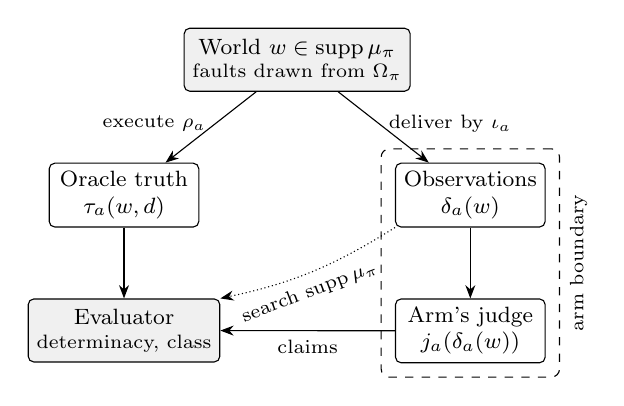
\begin{tikzpicture}[
  font=\footnotesize,
  box/.style={draw, rounded corners=2pt, align=center, minimum height=8mm, inner sep=3pt},
  lane/.style={draw, dashed, rounded corners=3pt, inner sep=5pt},
  >=Stealth]
\node[box, fill=black!6, minimum width=24mm] (world) {World $w \in \supp\mu_\pi$\\[-1pt]\scriptsize faults drawn from $\Omega_\pi$};
\node[box, below left=9mm and -2mm of world, minimum width=19mm] (truth) {Oracle truth\\$\truth_a(w,d)$};
\node[box, below right=9mm and -2mm of world, minimum width=19mm] (deliv) {Observations\\$\obs_a(w)$};
\node[box, below=9mm of deliv, minimum width=19mm] (judge) {Arm's judge\\$j_a(\obs_a(w))$};
\node[box, below=9mm of truth, minimum width=19mm, fill=black!6] (eval) {Evaluator\\[-1pt]\scriptsize determinacy, class};
\draw[->] (world) -- node[left, pos=.45]{\scriptsize execute $\rho_a$} (truth);
\draw[->] (world) -- node[right, pos=.45]{\scriptsize deliver by $\iota_a$} (deliv);
\draw[->] (deliv) -- (judge);
\draw[->] (truth) -- (eval);
\draw[->] (judge) -- node[below]{\scriptsize claims} (eval);
\draw[->, densely dotted] (deliv.south west) to[bend left=10] node[below, sloped, pos=.55]{\scriptsize search $\supp\mu_\pi$} (eval.north east);
\node[lane, fit=(deliv)(judge), label={[font=\scriptsize]right:\rotatebox{90}{arm boundary}}] {};
\end{tikzpicture}
\caption{The three records. The world executes the arm's protocol features $\rho_a$ to produce truth and delivers observations by the arm's interface $\iota_a$. The arm's judge sees only its observations. The evaluator holds truth, observations and claims apart and decides determinacy by searching the environment's support for worlds that give the arm the same observations.}
\label{fig:records}
\end{figure}

\subsection{Judgments}

A participant's claim about a dependency takes a value in
\[
\J = \{\Ful, \Vio, \Pen, \Ind\}.
\]
$\Ful$, $\Vio$ and $\Pen$ are \emph{definitive}; $\Ind$ is an abstention. $\Pen$ is the definitive claim that a dependency's deadline has not yet passed; every judgment in DMBench is made after every deadline, so $\Pen$ does not occur there. A judgment is never scored by accuracy alone: a judge that abstains on every difficult case is accurate on what it claims. Coverage, false definitive claims and correct abstention are reported separately~\cite{chow1970optimum,elyaniv2010foundations}.

\section{The Adequacy Calculus}
\label{sec:calculus}

\subsection{Environments, arms and runs}

\begin{definition}[Environment]
\label{def:environment}
An \emph{environment} for a scenario is a pair $\Omega_\pi = (W, \mu_\pi)$ of a set $W$ of worlds and a probability distribution $\mu_\pi$ on $W$ called a \emph{fault profile}. A world fixes every exogenous choice of a run: each participant's conduct, each message's fate and transit, each clock's skew, each read's freshness. Its \emph{support} $\supp\mu_\pi = \{ w \in W : \mu_\pi(w) > 0 \}$ is the set of admissible worlds.
\end{definition}

In DMBench every support is finite, and a world is a tuple of slot values; a profile assigns weights to each slot's values independently and a canonical map identifies worlds that differ only in slots that cannot matter (\cref{sec:method}).

\begin{definition}[Arm]
\label{def:arm}
An \emph{arm} for a scenario with dependencies $D$ is a triple $a = (\rho_a, \iota_a, j_a)$ of protocol features, an interface and a judge. Executing $a$ in world $w$ yields
\begin{itemize}
\item a truth assignment $\truth_a(w, \cdot) : D \to \{\Ful, \Vio\}$, whether each dependency's condition $\gamma$ held at evaluation; and
\item a delivery sequence $\obs_a(w) \in \Delta^*$, the observations the arm's participant receives, in arrival order.
\end{itemize}
The judge maps a delivery sequence to a claim per dependency, $j_a : \Delta^* \to (D \to \J \times 2^{\mathbb{N}})$, where the second component cites the indices of the deliveries the claim relies on.
\end{definition}

Truth depends on $\rho_a$; observations depend on $\rho_a$ and $\iota_a$; the judge sees only observations. Two arms in the same world can therefore differ in truth, in observations, or only in judgment, and each difference is a different kind of inadequacy (\cref{fig:factor}).

\subsection{Operational and epistemic adequacy}

\begin{definition}[Operational adequacy]
\label{def:opadeq}
Arm $a$ is \emph{operationally adequate} for $d$ under $\Omega_\pi$ when $\truth_a(w, d) = \Ful$ for every $w \in \supp\mu_\pi$. A world $w$ exhibits a \emph{protocol-induced violation} of $d$ for $a$ when $\truth_a(w,d) = \Vio$ and $\truth_b(w,d) = \Ful$ for some arm $b$ of the same scenario.
\end{definition}

Operational adequacy is rare when participants' conduct is exogenous: a provider that never accepts violates the handoff under every protocol. Protocol-induced violations isolate what the mechanism is responsible for.

\begin{definition}[Observation equivalence, determinacy]
\label{def:det}
Worlds $w, w' \in \supp\mu_\pi$ are \emph{observation-equivalent for $a$}, written $w \sim_a w'$, when $\obs_a(w) = \obs_a(w')$. Dependency $d$ is \emph{determined for $a$ at $w$} when $\truth_a(w', d) = \truth_a(w, d)$ for every $w' \sim_a w$. The \emph{determinable mass} of $a$ for $d$ under $\Omega_\pi$ is
\[
\dm_\pi(a, d) = \mu_\pi\{ w : d \text{ is determined for } a \text{ at } w \}.
\]
\end{definition}

\begin{definition}[Soundness, coverage]
\label{def:sound}
Write $j_a(w,d)$ for the judgment component of $j_a(\obs_a(w))(d)$. Judge $j_a$ is \emph{sound} for $d$ under $\Omega_\pi$ when, for every $w \in \supp\mu_\pi$, $j_a(w,d) \in \{\Ful, \Vio\}$ implies $j_a(w,d) = \truth_a(w,d)$. Its \emph{coverage} is $\cov_\pi(j_a, d) = \mu_\pi\{ w : j_a(w,d) \neq \Ind \}$.
\end{definition}

\begin{definition}[Epistemic and strong adequacy]
\label{def:epadeq}
Arm $a$ is \emph{epistemically adequate} for $d$ under $\Omega_\pi$ when $j_a$ is sound and $\cov_\pi(j_a, d) = 1$. It is \emph{strongly adequate} when it is both operationally and epistemically adequate.
\end{definition}

\begin{figure}[t]
\centering
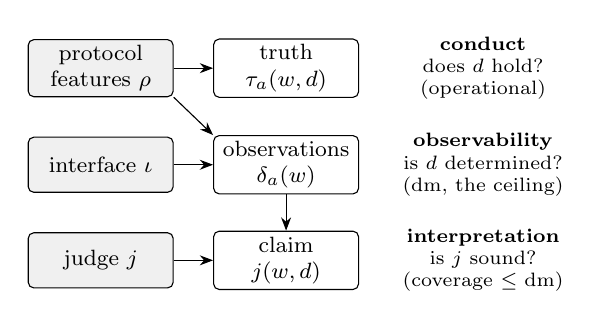
\begin{tikzpicture}[font=\footnotesize, >=Stealth,
  b/.style={draw, rounded corners=2pt, align=center, minimum height=7mm, inner sep=2pt, text width=17mm},
  q/.style={align=center, font=\scriptsize, text width=21mm}]
\node[b, fill=black!6] (rho) {protocol\\features $\rho$};
\node[b, right=5mm of rho] (tau) {truth\\$\truth_a(w,d)$};
\node[q, right=4mm of tau] (qa) {\textbf{conduct}\\does $d$ hold?\\(operational)};
\node[b, fill=black!6, below=5mm of rho] (iota) {interface $\iota$};
\node[b, right=5mm of iota] (del) {observations\\$\obs_a(w)$};
\node[q, right=4mm of del] (qb) {\textbf{observability}\\is $d$ determined?\\($\dm$, the ceiling)};
\node[b, fill=black!6, below=5mm of iota] (j) {judge $j$};
\node[b, right=5mm of j] (cl) {claim\\$j(w,d)$};
\node[q, right=4mm of cl] (qc) {\textbf{interpretation}\\is $j$ sound?\\(coverage $\le \dm$)};
\draw[->] (rho) -- (tau);
\draw[->] (iota) -- (del);
\draw[->] (rho.south east) -- (del.north west);
\draw[->] (j) -- (cl);
\draw[->] (del) -- (cl);
\end{tikzpicture}
\caption{Adequacy factors into three separately measurable parts. Protocol features decide conduct and so truth; features and interface together decide observations and so the ceiling on sound judgment; the judge decides only whether that ceiling is approached soundly.}
\label{fig:factor}
\end{figure}

Strong adequacy is the framework's original definition, $\forall r \in \mathrm{Runs}(P, \Omega) : \mathrm{Safe}(r, G) \wedge \mathrm{Resolve}(r, d) \wedge \mathrm{Observable}(r, d, E)$, read in a finite model: every run terminates in a judgment instant after every deadline (resolution), the dependency holds (operational safety), and the observer can establish it (observability with a sound judgment). It is deliberately demanding; DMBench measures distance from it rather than its attainment.

\subsection{Axioms}

The theory's commitments are stated as six axioms. Each has a formal reading in the calculus and a measurable consequence in DMBench.

\begin{axiom}[Dependency specificity]
\label{ax:specificity}
Adequacy is defined relative to a dependency. In the calculus every adequacy predicate takes $d$ as an argument; a protocol has no adequacy simpliciter.
\end{axiom}

\begin{axiom}[Assumption relativity]
\label{ax:assumption}
Changing the admissible environment can change adequacy. Determinacy quantifies over $\supp\mu_\pi$: enlarging the support can only shrink the set of worlds at which a dependency is determined, and a judge sound under one support need not be sound under a larger one (\cref{prop:support}).
\end{axiom}

\begin{axiom}[Semantic non-equivalence]
\label{ax:nonequivalence}
Evidence of a valid message exchange, a valid state transition and a discharged obligation are not interchangeable without an explicit, sound mapping. In the calculus, a message, a record entry and a truth value are different objects, and a judge's mapping from the first two to the third is what soundness constrains.
\end{axiom}

\begin{axiom}[Responsibility continuity]
\label{ax:continuity}
For every dependency requiring accountable ownership, a discharge, transfer or termination of responsibility must be evidenced; delegation does not extinguish the original obligation. DMBench measures the time responsibility is unowned as the accountability gap rate.
\end{axiom}

\begin{axiom}[Evidence soundness]
\label{ax:evidence}
An observer may assert a definitive outcome only when its evidence supports it under the declared observation semantics; otherwise the judgment is $\Ind$. In the calculus this is \cref{def:sound}.
\end{axiom}

\begin{axiom}[Nontrivial composition]
\label{ax:composition}
Adequacy of two protocols separately does not imply adequacy of their composition without interface, responsibility and observability conditions. \Cref{thm:p2} states the observability condition.
\end{axiom}

\subsection{Indistinguishability and the ceiling on sound judgment}

\begin{theorem}[Indistinguishability]
\label{thm:p1}
If $w_1 \sim_a w_2$ and $\truth_a(w_1, d) \neq \truth_a(w_2, d)$, then for every judge $j$ over $a$'s observations, either $j$ abstains on $d$ at both $w_1$ and $w_2$, or $j$ makes a false definitive claim about $d$ at one of them.
\end{theorem}

\begin{proof}
$j$ is a function of $\obs_a(w)$, and $\obs_a(w_1) = \obs_a(w_2)$, so $j(w_1, d) = j(w_2, d)$. If this value is definitive it equals at most one of the two distinct truth values.
\end{proof}

The theorem is the framework's proposition P1 (\cref{fig:ceiling}). Its content is not the proof, which is immediate, but its consequence: a message saying ``completed'' cannot establish completion unless the observation model separates the worlds in which it is sent truthfully from those in which it is not. DMBench finds witness pairs in seven of the eight families (\cref{tab:p1}).

\begin{theorem}[Ceiling on sound judgment]
\label{thm:ceiling}
For every arm $a$, dependency $d$ and environment $\Omega_\pi$:
\begin{enumerate}
\item every judge $j$ sound for $d$ satisfies $\cov_\pi(j, d) \leq \dm_\pi(a, d)$; and
\item the canonical judge $j^\star_a$, which returns the common truth value of $d$ over the observation class of its input when that value is unique and $\Ind$ otherwise, is sound and satisfies $\cov_\pi(j^\star_a, d) = \dm_\pi(a, d)$.
\end{enumerate}
\end{theorem}

\begin{proof}[Proof sketch]
If a sound $j$ is definitive at $w$, it returns the same value at every $w' \sim_a w$, and soundness forces that value to equal $\truth_a(w', d)$ for each; so $d$ is determined at $w$. Integrating over $\mu_\pi$ gives (1). $j^\star_a$ is well defined because its input determines the class, sound by construction, and definitive exactly where $d$ is determined, giving (2). The full proof is in \cref{app:proofs}.
\end{proof}

\begin{figure}[t]
\centering
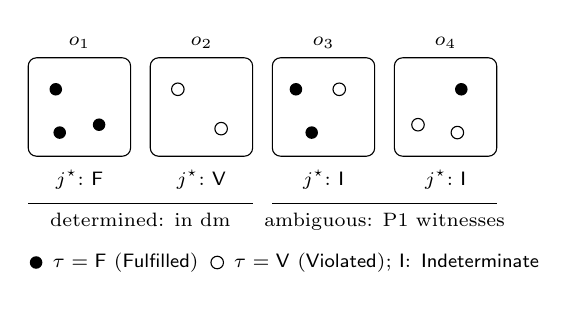
\begin{tikzpicture}[font=\scriptsize, >=Stealth]
\tikzset{f/.style={circle, fill=black, inner sep=1.6pt}, v/.style={circle, draw, fill=white, inner sep=1.6pt}}
\foreach \x/\lab/\kind in {0/{$o_1$}/a, 1.55/{$o_2$}/b, 3.1/{$o_3$}/c, 4.65/{$o_4$}/d}{
  \draw[rounded corners=3pt] (\x,0) rectangle ++(1.3,1.25);
  \node[anchor=south] at (\x+0.65,1.25) {\lab};
}
\node[f] at (0.35,0.85) {}; \node[f] at (0.9,0.4) {}; \node[f] at (0.4,0.3) {};
\node[v] at (1.9,0.85) {}; \node[v] at (2.45,0.35) {};
\node[f] at (3.4,0.85) {}; \node[v] at (3.95,0.85) {}; \node[f] at (3.6,0.3) {};
\node[v] at (4.95,0.4) {}; \node[f] at (5.5,0.85) {}; \node[v] at (5.45,0.3) {};
\node at (0.65,-0.3) {$j^\star{:}\ \mathsf{F}$};
\node at (2.2,-0.3) {$j^\star{:}\ \mathsf{V}$};
\node at (3.75,-0.3) {$j^\star{:}\ \mathsf{I}$};
\node at (5.3,-0.3) {$j^\star{:}\ \mathsf{I}$};
\draw (0,-0.6) -- (2.85,-0.6) node[midway, below]{determined: in $\dm$};
\draw (3.1,-0.6) -- (5.95,-0.6) node[midway, below]{ambiguous: P1 witnesses};
\node[f, label=right:{$\truth = \mathsf{F}$ ($\Ful$)}] at (0.1,-1.35) {};
\node[v, label=right:{$\truth = \mathsf{V}$ ($\Vio$); $\mathsf{I}$: $\Ind$}] at (2.4,-1.35) {};
\end{tikzpicture}
\caption{Worlds of a support grouped by the observations an arm receives. A sound judge can be definitive only on truth-constant classes ($o_1$, $o_2$); on mixed classes ($o_3$, $o_4$) every definitive claim is false somewhere (\cref{thm:p1}). The canonical judge $j^\star$ is definitive exactly on the truth-constant classes, so its coverage is the determinable mass (\cref{thm:ceiling}).}
\label{fig:ceiling}
\end{figure}

\begin{corollary}[Epistemic adequacy is a property of the interface]
\label{cor:interface}
Arm $a$ admits an epistemically adequate judge for $d$ under $\Omega_\pi$ if and only if $\dm_\pi(a, d) = 1$. For a sound judge $j$, the shortfall $\dm_\pi(a,d) - \cov_\pi(j,d) \geq 0$ is exactly the mass of its abstentions on determined outcomes.
\end{corollary}

DMBench reports that shortfall as the class \emph{abstained-miss}. A sound judge with no abstained-miss is optimal for its observations; a protocol whose determinable mass is below one cannot be made epistemically adequate by a better judge, only by a richer interface.

\begin{proposition}[Monotonicity]
\label{prop:monotone}
If two arms share protocol features, so that $\truth_a = \truth_b$, and $\obs_a = h \circ \obs_b$ for some function $h$ (arm $b$ observes at least what $a$ observes), then $d$ determined for $a$ at $w$ implies $d$ determined for $b$ at $w$, and $\dm_\pi(b, d) \geq \dm_\pi(a, d)$.
\end{proposition}

\begin{proposition}[Support relativity]
\label{prop:support}
Let $\supp\mu \subseteq \supp\mu'$. A judge sound under $\mu'$ is sound under $\mu$, and if $d$ is determined for $a$ at $w$ under $\mu'$ then it is determined at $w$ under $\mu$. The converses fail.
\end{proposition}

\Cref{prop:support} is the formal content of \cref{ax:assumption} and a caution for benchmark design: determinacy, and so the class abstained-miss, is relative to the modelled support. An abstention can be a miss in a narrow model and correct in the world the paradigm assumes (\cref{sec:limitations}).

\subsection{Composition}

Consider a composition in which an observer $H$ depends on a party $S$ that it does not observe directly, through a relay $V$ that does: $H \leftarrow V \leftarrow S$. Let $s$ range over the reachable composite states, $t(s)$ be the truth of $H$'s dependency, $\sigma(s)$ be what $V$ records about $S$, and $H$'s observation be $\obs(s) = \kappa(\sigma(s), v(s))$, where $v(s)$ is the rest of what $H$ observes and $\kappa$ combines them.

\begin{definition}[Compliance-decidability]
A composition is \emph{compliance-decidable} for $H$ when $\dm = 1$ for $H$'s dependency, equivalently (\cref{cor:interface}) when $H$ admits a sound judge with full coverage.
\end{definition}

\begin{theorem}[Composition requires distinguishability]
\label{thm:p2}
A composition is compliance-decidable for $H$ if and only if $\obs$ separates every pair of reachable states with different truth. In particular, if there are reachable $s, s'$ with $t(s) \neq t(s')$, $\sigma(s) = \sigma(s')$ and $v(s) = v(s')$, the composition is not compliance-decidable for $H$, however fine $H$'s observation of $V$ is.
\end{theorem}

The first part is \cref{thm:ceiling} applied to the composite; the second follows because $\kappa$ cannot separate what its arguments do not. The design consequence is the framework's proposition P2: either the observation model distinguishes all compliance-relevant reachable states, or the judgment set must include $\Ind$. The second part sharpens it. Refining $H$'s view of $V$ from a coarse case status to $V$'s full record of $S$'s stage does not suffice when $\sigma$ is $S$'s own report, because a premature report and an on-time start produce the same record; DMBench measures determinable mass rising from 0 to 1 with honest reporting, falling to 0.25 when reports can be premature, and returning to 1 with an attestation of $S$'s start (\cref{tab:p2}).

\subsection{Refinement}

\begin{theorem}[Conditional preservation under refinement]
\label{thm:p3}
Let $a'$ be a variant of arm $a$ for dependency $d$ under $\Omega_\pi$.
\begin{enumerate}
\item If $\rho_{a'} = \rho_a$ and $\iota_{a'} = \iota_a$, then $\dm_\pi(a', d) = \dm_\pi(a, d)$ and $a'$ is epistemically adequate exactly when its judge is sound with full coverage: adequacy can change only through interpretation.
\item If $\rho_{a'} = \rho_a$ and $\obs_a = h \circ \obs_{a'}$, then $\dm_\pi(a', d) \geq \dm_\pi(a, d)$: a refinement that keeps every observation cannot lose determinacy.
\item If $\rho_{a'} = \rho_a$ and $\obs_{a'} = h \circ \obs_a$ with $h$ not injective on the range of $\obs_a$, then $\dm_\pi(a', d)$ can be strictly smaller: a refinement that drops observations can lose determinacy even when it removes every bad execution.
\item If $\rho_{a'} \neq \rho_a$, then $\truth_{a'}$ can differ from $\truth_a$ in either direction, and soundness of $j_a$ implies nothing about soundness of the same judge for $a'$.
\end{enumerate}
\end{theorem}

Each clause is witnessed in DMBench, so none of the four conditions the framework lists for preservation (safety invariants, resolution behaviour, observations, normative interpretation) can be dropped. Clause (1): the hybrid's ablation shares the hybrid's protocol and interface in seven families and loses safety in all seven with no loss of observation. Clauses (2) and (3): the composition family's observation models satisfy the precondition exactly, since the coarse case status is a projection of the staged record and the staged record a projection of the staged record with attestation; determinable mass for the stage dependency moves monotonically between 0 and 1 across them (\cref{tab:p2}). The single-paradigm arms that share the hybrid's protocol features but have smaller interfaces lose determinacy on between 34 and 251 world--dependency pairs per family. Clause (4): in the reservation family the ablation also drops the hybrid's fencing tokens, which changes conduct, and it loses both safety and observation (\cref{tab:p3}).

\subsection{The hybrid's correctness condition}

The framework states the hybrid's correctness as a conjunction $\mathrm{Correct}_H = C_I \wedge C_B \wedge C_N \wedge C_E$ of communication conformance, behavioural safety and progress, normative consistency, and evidence soundness and observability, and notes that the conjunction requires cross-layer consistency. The calculus makes $C_E$ precise: it is soundness of $j_H$ together with high determinable mass of $\iota_H$. DMBench's hybrid implements $C_E$ by three rules (\cref{sec:dmbench}): a participant's report of its own performance is not evidence of that performance; a record is authoritative only up to the instant through which it is complete; otherwise the judgment is $\Ind$. The ablation removes exactly these rules.

\section{Executable Semantics}
\label{sec:method}

The calculus is built as executable semantics in Racket with PLT Redex~\cite{felleisen2009redex}, following the practice of mechanizing a semantics before trusting it~\cite{klein2012run}. Each object of \cref{sec:calculus} has one executable counterpart, and every number reported in \cref{sec:results} is computed by the code, not transcribed.

\subsection{Languages}

A base language $\mathrm{DMAT_0}$ fixes what every scenario shares: instants as natural numbers, the judgment set $\J$, claims $(\mathtt{claim}\ d\ J\ (i\ldots))$ and the three forms of delivery:
\[
\begin{array}{rcl}
\delta & ::= & (\mathtt{msg}\ M\ t_{\mathit{arr}}\ t_{\mathit{asr}}\ \mathit{payload}\ldots) \\
       & \mid & (\mathtt{read\text{-}ok}\ t\ \mathit{view}) \;\mid\; (\mathtt{read\text{-}failed}\ t)
\end{array}
\]
A message carries its arrival instant and the instant its sender asserts for it, which is the event it reports or the sender's clock; the two differ under transit delay and clock skew, and arms that confuse them are the arms that fail under those faults. Each scenario family extends $\mathrm{DMAT_0}$ with its own worlds, record views and message kinds, so that each family's terms form a closed language and every world, delivery sequence and claim is checked against it (\cref{fig:arch}).

\begin{figure}[t]
\centering
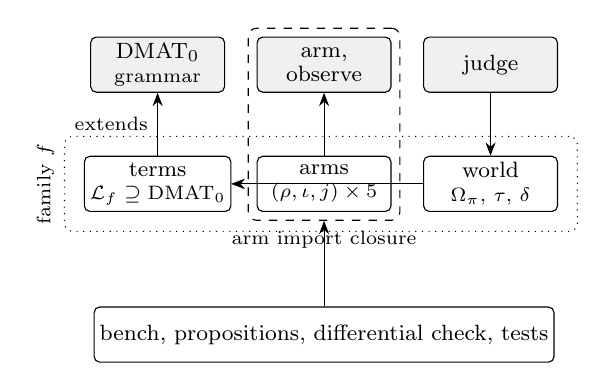
\begin{tikzpicture}[
  font=\footnotesize, >=Stealth,
  m/.style={draw, rounded corners=2pt, align=center, minimum width=17mm, minimum height=7mm, inner sep=2pt},
  core/.style={m, fill=black!6}]
\node[core] (g) {$\mathrm{DMAT_0}$\\[-1pt]\scriptsize grammar};
\node[core, right=4mm of g] (arm) {arm,\\[-1pt]observe};
\node[core, right=4mm of arm] (judge) {judge};
\node[m, below=8mm of g] (terms) {terms\\[-1pt]\scriptsize $\mathcal{L}_f \supseteq \mathrm{DMAT_0}$};
\node[m, below=8mm of arm] (arms) {arms\\[-1pt]\scriptsize $(\rho,\iota,j)\times 5$};
\node[m, below=8mm of judge] (world) {world\\[-1pt]\scriptsize $\Omega_\pi$, $\truth$, $\obs$};
\draw[->] (terms) -- node[left]{\scriptsize extends} (g);
\draw[->] (arms) -- (terms);
\draw[->] (arms) -- (arm);
\draw[->] (world) -- (terms);
\draw[->] (judge) -- (world.north);
\node[draw, dashed, rounded corners=3pt, fit=(arms)(arm), inner sep=3pt, label={[font=\scriptsize, align=center]below:arm import closure}] (iso) {};
\node[draw, dotted, rounded corners=3pt, fit=(terms)(arms)(world), inner sep=7pt, label={[font=\scriptsize]left:\rotatebox{90}{family $f$}}] {};
\node[m, below=12mm of arms, minimum width=50mm] (bench) {bench, propositions, differential check, tests};
\draw[->] (bench) -- (iso.south);
\end{tikzpicture}
\caption{Module structure of the executable models. Each family extends the base grammar with its own closed language. An arm module may import only the core arm and observe modules and its family's terms; the world and the judge are outside its import closure, which a test checks for every arm, including a planted leak the check must catch.}
\label{fig:arch}
\end{figure}

\subsection{Families as data}

A family is a record of its dependencies with their kinds; its world slots; base weights for each slot's values; its fault profiles as overrides of those weights; a canonical map that identifies worlds differing only in slots that cannot matter (a reply delay is irrelevant when no reply is sent); and two functions, \emph{execute}, which runs an arm's protocol features in a world and returns truth, unowned-responsibility time and required-responsibility time, and \emph{deliver}, which returns the arm's delivery sequence. Only world modules construct families.

\subsection{Oracle isolation}

An arm is a record $(\rho, \iota, j)$. The world reads $\rho$ and $\iota$; the judge $j$ receives only the delivery sequence. Isolation is enforced structurally: a test computes the transitive closure of every arm module's imports and fails if it reaches anything beyond the core arm, observe and grammar modules and the family's own terms. The test is itself tested by planting an arm that imports a world module.

\subsection{Determinacy by exhaustive search}

The judge enumerates each profile's support, computes every arm's delivery sequence in every world, and groups worlds by delivery sequence. A dependency is determined for an arm at a world when every world in its group has the same truth (\cref{def:det}). Each claim is then classified:

\begin{center}
\small
\begin{tabular}{@{}ll@{}}
\toprule
Class & Condition \\
\midrule
supported & definitive, true, determined, citing a delivery \\
lucky & definitive and true, but not determined or uncited \\
false & definitive and not true \\
abstained-ok & $\Ind$, and not determined \\
abstained-miss & $\Ind$, though determined \\
\bottomrule
\end{tabular}
\end{center}

\subsection{Metrics}

For arm $a$ under profile $\pi$, with expectations taken exactly over $\mu_\pi$:
\begin{itemize}
\item the \emph{safety failure rate} $\mathrm{SFR}$ is the probability that a run contains a false claim about any dependency;
\item the \emph{false-completion rate} $\mathrm{FCR}$ is the expected number of $\Ful$ claims that are false or lucky, divided by the expected number of $\Ful$ claims;
\item the \emph{accountability gap rate} $\mathrm{AGR}$ is the expected time responsibility is owned by nobody, divided by the expected time responsibility is required, both computed by the world's execution;
\item \emph{coverage} is the share of claims that are definitive, and each class's share is reported, with \emph{determinable} the share of claims whose outcome the observations determine.
\end{itemize}
FCR counts lucky claims as well as false ones: a completion claim that happens to be true without evidence is an unsupported claim of completion.

\subsection{Exact expectation and seeded sampling}

Because supports are finite, every metric is computed as an exact rational expectation. Sampled runs exist to check the exact computation and to produce per-run records. A world is drawn per slot by a keyed hash, $\mathrm{SHA\text{-}256}(\text{family}, \text{seed}, \text{profile}, \text{slot})$, so a seed fixes the same world for every arm (common random numbers), and a draw for one slot never shifts another. With 100 seeds per family and profile (18,000 runs), the worst deviation of sampled SFR from its exact value is 2.7 standard errors over 180 cells, none beyond 3; every run is written with its world, deliveries, claims and classification, and repeated runs produce byte-identical output.

\subsection{Tests}

Twenty-nine tests cover: well-formedness of every world, delivery sequence and claim against its family's language; totality of execution, delivery and every judge on worlds generated from each grammar; idempotence of the canonical maps; oracle isolation with a planted leak; determinism and common random numbers; a brute-force recomputation of every classification; the family-specific properties the benchmark is built to exhibit; propositions P1--P3; and the independent-authorship results of \cref{sec:independent}.

\section{DMBench}
\label{sec:dmbench}

DMBench asks four questions of each protocol: can it represent the coordination obligation; can it preserve required behaviour under failure; can participants recover without losing safety or accountability; and can an independent observer determine what happened. It separates a failure of a protocol family from a failure of a particular implementation by giving every arm the same scenario, the same faults on the same abstract interactions, and the same judge.

\subsection{Scenario families}

\Cref{tab:families} lists the eight families. Each is specified by its dependencies' success conditions, its timeline, the conduct its participants may exhibit and its faults; \cref{app:families} gives the full specifications. In four families the arms' protocol features decide conduct, so truth depends on the arm.

\begin{table*}[t]
\centering
\caption{DMBench scenario families. Kinds: Fl flow, Sh sharing, Fi fit, Te temporal. Worlds counts the canonical worlds summed over the family's profiles.}
\label{tab:families}
\footnotesize
\setlength{\tabcolsep}{4pt}
\begin{tabular}{@{}l p{52mm} p{40mm} p{42mm} r r@{}}
\toprule
Family & Scenario & Dependencies & Conduct-affecting protocol feature & Prof. & Worlds \\
\midrule
\family{handoff} & Hospital $H$ refers a patient to provider $V$; $V$ may accept late or not at all, crash, or report a start prematurely & \texttt{flow} (Fl): accepted by the deadline; \texttt{temporal} (Te): care initiated & --- & 7 & 694 \\
\family{reservation} & Allocator grants one resource to $h_1$ under a lease; $h_2$ requests it; $h_1$ releases, overruns or dies & \texttt{sharing} (Sh): never two effective users; \texttt{temporal} (Te): $h_2$ granted by $D_2$ & regrant on release; on expiry; on expiry with fencing tokens & 4 & 32 \\
\family{agreement} & Buyer $B$ and seller $S$; $S$ may alter terms or revoke concurrently with $B$'s confirmation & \texttt{fit} (Fi): nobody bound to unfitting terms; \texttt{mutual} (Fl): both bound or neither & whether $B$ checks fit; when $B$ is bound (on send, on acknowledgement, or reconciled) & 5 & 100 \\
\family{delegation} & $V$ without capacity delegates to $S$, which accepts or declines & \texttt{continuity} (Fl): never unowned; \texttt{temporal} (Te) & delegating releases $V$, or $V$ retains until $S$ accepts & 4 & 182 \\
\family{deadline} & $V$ owes a service by a deadline and reports completion stamped by its own clock & \texttt{temporal} (Te) in true time; \texttt{completion} (Fl) & --- & 4 & 65 \\
\family{external} & $V$ performs part A and dispatches part B to an executor $X$ outside the protocol & \texttt{internal} (Fl): A performed; \texttt{external} (Fl): B performed in full & --- & 4 & 62 \\
\family{composition} & $H \leftarrow V \leftarrow S$ across three organizations; $H$ has no protocol with $S$ & \texttt{temporal} (Te): $S$ started by the deadline; \texttt{delivery} (Fl) & --- (observation model of $V$'s case varies) & 4 & 76 \\
\family{replacement} & $V$ may withdraw; $V_2$ accepts or declines; a withdrawn $V$ may emit a stale START & \texttt{continuity} (Fl); \texttt{temporal} (Te) & withdrawal releases $V$, or $V$ retains until $V_2$ accepts & 4 & 172 \\
\bottomrule
\end{tabular}
\end{table*}

\subsection{Faults}

The framework's fault matrix lists nine faults. \Cref{tab:faults} records where each is modelled. Timing varies per run: late conduct, slow replies that arrive after later messages, transit delay, clock skew, stale queued messages and interleavings of concurrent events are all world choices. Time is discrete and each variation is enumerated.

\begin{table}[t]
\centering
\caption{The framework's fault matrix as modelled.}
\label{tab:faults}
\small
\begin{tabular}{@{}p{24mm} p{56mm}@{}}
\toprule
Fault & Where modelled \\
\midrule
Lost reply & every family: acceptances, notices, attestations, receipts, confirmations, acknowledgements, releases \\
Duplicate command & duplicated acceptance (\family{handoff}) \\
Stale observation & stale reads (five families); record lag with a watermark (\family{handoff}, \family{external}); a stale queued message (\family{replacement}) \\
Concurrent updates & revocation and confirmation crossing in both orders (\family{agreement}); two users of one resource (\family{reservation}) \\
Resource exhaustion & $V$ without capacity (\family{delegation}) \\
Conflicting acceptance & altered terms; crossing confirmation and revocation (\family{agreement}) \\
Deadline expiry & care, service and stage deadlines; lease expiry \\
Actor disappears & crash after acceptance; a holder dying with its lease; withdrawal; a subcontractor declining \\
Evidence contradiction & premature start report; premature completion report; a subcontractor's premature self-report; clock skew; the stale queued message \\
\bottomrule
\end{tabular}
\end{table}

\subsection{Arms}

Each family has five arms, each written as a faithful practitioner of its paradigm would write it.

\paragraph{\arm{Chor}} A global type projected to the observer. The observer's knowledge is its session: the messages of its projection, and where defined a read-back of the counterpart's session log. Timed branches fire on arrival, and when the branch for a missing or late message fires the session records the partner's failure. Messages are checked by type, not payload value. Facts outside the projection are $\Ind$.

\paragraph{\arm{Fsm}} Communicating state machines with guards and timeouts on each participant's own clock. A received message that moves the counterpart to a final state takes precedence over a record; otherwise the counterpart's state record is authoritative and taken as current.

\paragraph{\arm{Comm}} Commitments with the lifecycle conditional, detached, discharged, violated, released, delegated and pending. Judgments are the commitment's state as the creditor holds it; a commitment the creditor has not seen discharged by its deadline is violated.

\paragraph{\arm{Hybrid}} Commitments in which responsibility is retained or assigned but never dropped, state-machine guards and records, and an evidentiary discipline of three rules:
\begin{enumerate}
\item[E1] A participant's report of its own performance, in a message or a record entry, is not evidence of that performance; a $\Ful$ claim needs an attestation from another party, a third party's record or a trusted clock. A participant's report of not having performed can establish a negative.
\item[E2] A record is authoritative for an event only if its completeness watermark covers the instant by which the event would have been recorded.
\item[E3] Otherwise the judgment is $\Ind$.
\end{enumerate}
Responsibility continuity is judged from the commitment structure, not from reports of performance. Guarantees checked by an independent party, such as fencing tokens checked by a resource~\cite{kleppmann2017designing}, are evidence.

\paragraph{\arm{Hybrid-noE}} The ablation, abbreviated \arm{Hyb-noE} in tables: the hybrid with E1--E3 removed. Reports count as evidence; every successful read is authoritative, including over messages; where the hybrid would abstain, the commitment rule applies. In \family{reservation} the ablation also drops the fencing tokens.

The arms' interfaces differ only where the paradigm defines different observables: the hybrid's protocols define an independent attestation or receipt and a full record view with a watermark; the others define the messages and record views their paradigm has. Every arm receives the same faults on the interactions it shares with the others.

\section{Independent Authorship and Differential Adjudication}
\label{sec:independent}

A benchmark whose arms are written by one author measures that author's reading of each paradigm. The framework's validity design asks for protocol authors separate from evaluator authors~\cite{avizienis1985nversion}. DMBench meets that requirement with a differential protocol (\cref{fig:diff}).

\begin{figure}[t]
\centering
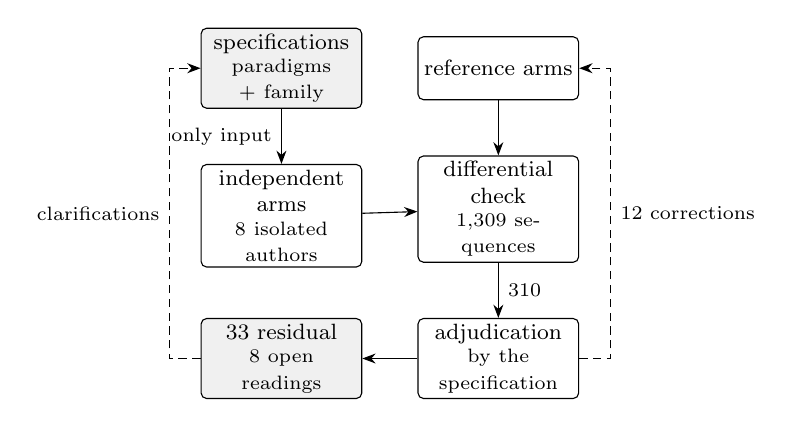
\begin{tikzpicture}[
  font=\footnotesize, >=Stealth,
  b/.style={draw, rounded corners=2pt, align=center, minimum height=8mm, inner sep=2pt, text width=19mm}]
\node[b, fill=black!6] (spec) {specifications\\[-1pt]\scriptsize paradigms + family};
\node[b, below=7mm of spec] (ind) {independent arms\\[-1pt]\scriptsize 8 isolated authors};
\node[b, right=7mm of spec] (ref) {reference arms};
\node[b, below=7mm of ref] (diff) {differential check\\[-1pt]\scriptsize 1,309 sequences};
\node[b, below=7mm of diff] (adj) {adjudication\\[-1pt]\scriptsize by the specification};
\node[b, left=7mm of adj, fill=black!6] (res) {33 residual\\[-1pt]\scriptsize 8 open readings};
\draw[->] (spec) -- node[left]{\scriptsize only input} (ind);
\draw[->] (ind) -- (diff);
\draw[->] (ref) -- (diff);
\draw[->] (diff) -- node[right]{\scriptsize 310} (adj);
\draw[->] (adj) -- (res);
\draw[->, densely dashed] (adj.east) -- ++(4mm,0) |- node[pos=0.25, right]{\scriptsize 12 corrections} (ref.east);
\draw[->, densely dashed] (res.west) -- ++(-4mm,0) |- node[pos=0.25, left]{\scriptsize clarifications} (spec.west);
\end{tikzpicture}
\caption{The differential protocol. Independent authors write arms from the specifications alone. Every reachable observation sequence is judged by both sets of arms; each disagreement is traced to a cause and decided by the written specification. Reference departures are corrected in the reference; open questions are clarified in a dated addition to the specification and reported as residue. Independent arms are never edited.}
\label{fig:diff}
\end{figure}

\subsection{Protocol}

A specification of the arm contract and the five paradigms, and one specification per family stating its scenario, dependencies, constants, conduct, faults, delivery rules, record views and each arm's fixed protocol features and interface, were written before the comparison. For each family a separate author received only these specifications, the core arm and observe modules and the family's terms module, in a workspace without the reference arms, the world modules or any earlier version, with instructions to read nothing else. Each author wrote five judges and a domain comment for each, and verified totality with a checker built by hand from the specification's fault model.

The comparison runs both sets of judges on every distinct delivery sequence that any profile of any family produces: 1,309 sequences over the forty family--arm pairs. Because protocol features and interfaces are fixed by the specification, both arms of a name receive the same deliveries in every world, so any difference is a difference of judgment, and agreement on a sequence is agreement on every world that produces it.

\subsection{Adjudication}

The first comparison disagreed on 310 sequences. Each disagreement was traced to a cause and decided by one rule: the written specification is the contract. Twelve causes were departures of the reference arms from the specification and were corrected in the reference; among them, choreography timeouts treated as violations, arrival-based bounds, E1 applied to a participant's records as well as its messages, continuity judged from the commitment structure, the ablation retaining the commitment rule, and responsibility evaluated at each message's instant so that a withdrawn participant's stale message is not credited. Eight causes were readings the specification left open and both of which are defensible paradigm practice; for these the reference reading was kept, the specification received a dated clarification, and the residue is reported (\cref{tab:diff}; \cref{app:adjudication} lists every cause).

\begin{table}[t]
\centering
\caption{Differential check. Sequences: distinct delivery sequences over the family's five arms. Initial and residual: sequences judged differently before and after adjudication.}
\label{tab:diff}
\small
\begin{tabular}{@{}lrrr@{}}
\toprule
Family & Sequences & Initial & Residual \\
\midrule
\family{handoff} & 514 & 56 & 0 \\
\family{reservation} & 38 & 9 & 0 \\
\family{agreement} & 78 & 24 & 9 \\
\family{delegation} & 167 & 64 & 8 \\
\family{deadline} & 178 & 3 & 1 \\
\family{external} & 75 & 34 & 7 \\
\family{composition} & 61 & 26 & 8 \\
\family{replacement} & 198 & 94 & 0 \\
\midrule
Total & 1,309 & 310 & 33 \\
\bottomrule
\end{tabular}
\end{table}

\subsection{What the independent arms confirm}

Three results hold for the independent arms as written, before any change to the reference: the independent hybrid makes no false claim in any family under any profile; the independent ablation is unsafe in every family; and every independent single-paradigm arm is unsafe in some family. The cross-family conclusions of \cref{sec:results} therefore do not depend on the reference author's reading. Per-cell figures for single-paradigm arms do: under the independent reading of \family{agreement}, \arm{Chor} checks the payload of the seller's acceptance and is safe under reliable delivery, while under the reference reading it checks types only and has SFR 0.25. Both are reported.

\subsection{What the protocol does not establish}

The independent authors were separate agent instances of the same model family as the reference author. They did not see the reference arms or the world, so the check catches judgment errors and specification-to-code slips, and it found twelve. Agreement after adjudication shows that the specification determines the arms up to eight documented choices. It does not provide the diversity of separate human teams, and Knight and Leveson's finding that independently written versions share failures more often than independence predicts~\cite{knight1986experimental} applies with more force to authors trained alike.

\section{Results}
\label{sec:results}

All figures in this section are exact expectations over each profile's support. \Cref{fig:heat} gives each arm's worst safety failure rate over each family's profiles; \cref{tab:adv} gives the adversarial profile, which admits every fault the family models. \Cref{app:results} lists all 180 family--profile--arm rows.

\begin{figure}[t]
\centering
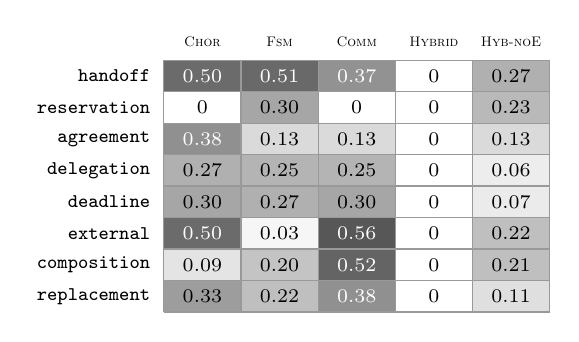
\begin{tikzpicture}[font=\scriptsize]
\node[anchor=south, font=\tiny] at (0.49,0.05) {\arm{Chor}};
\node[anchor=south, font=\tiny] at (1.47,0.05) {\arm{Fsm}};
\node[anchor=south, font=\tiny] at (2.45,0.05) {\arm{Comm}};
\node[anchor=south, font=\tiny] at (3.4299999999999997,0.05) {\arm{Hybrid}};
\node[anchor=south, font=\tiny] at (4.41,0.05) {\arm{Hyb-noE}};
\node[anchor=east] at (-0.05,-0.2) {\texttt{handoff}};
\fill[black!58.099999999999994] (0,-0.4) rectangle (0.98,0.0);
\node[text=white] at (0.49,-0.2) {0.50};
\fill[black!58.8] (0.98,-0.4) rectangle (1.96,0.0);
\node[text=white] at (1.47,-0.2) {0.51};
\fill[black!42.699999999999996] (1.96,-0.4) rectangle (2.94,0.0);
\node[text=white] at (2.45,-0.2) {0.37};
\fill[black!0] (2.94,-0.4) rectangle (3.92,0.0);
\node[text=black] at (3.4299999999999997,-0.2) {0};
\fill[black!30.799999999999997] (3.92,-0.4) rectangle (4.9,0.0);
\node[text=black] at (4.41,-0.2) {0.27};
\node[anchor=east] at (-0.05,-0.6000000000000001) {\texttt{reservation}};
\fill[black!0] (0,-0.8) rectangle (0.98,-0.4);
\node[text=black] at (0.49,-0.6000000000000001) {0};
\fill[black!35.0] (0.98,-0.8) rectangle (1.96,-0.4);
\node[text=black] at (1.47,-0.6000000000000001) {0.30};
\fill[black!0] (1.96,-0.8) rectangle (2.94,-0.4);
\node[text=black] at (2.45,-0.6000000000000001) {0};
\fill[black!0] (2.94,-0.8) rectangle (3.92,-0.4);
\node[text=black] at (3.4299999999999997,-0.6000000000000001) {0};
\fill[black!27.299999999999997] (3.92,-0.8) rectangle (4.9,-0.4);
\node[text=black] at (4.41,-0.6000000000000001) {0.23};
\node[anchor=east] at (-0.05,-1.0000000000000002) {\texttt{agreement}};
\fill[black!43.4] (0,-1.2000000000000002) rectangle (0.98,-0.8000000000000002);
\node[text=white] at (0.49,-1.0000000000000002) {0.38};
\fill[black!14.7] (0.98,-1.2000000000000002) rectangle (1.96,-0.8000000000000002);
\node[text=black] at (1.47,-1.0000000000000002) {0.13};
\fill[black!14.7] (1.96,-1.2000000000000002) rectangle (2.94,-0.8000000000000002);
\node[text=black] at (2.45,-1.0000000000000002) {0.13};
\fill[black!0] (2.94,-1.2000000000000002) rectangle (3.92,-0.8000000000000002);
\node[text=black] at (3.4299999999999997,-1.0000000000000002) {0};
\fill[black!14.7] (3.92,-1.2000000000000002) rectangle (4.9,-0.8000000000000002);
\node[text=black] at (4.41,-1.0000000000000002) {0.13};
\node[anchor=east] at (-0.05,-1.4000000000000001) {\texttt{delegation}};
\fill[black!30.799999999999997] (0,-1.6) rectangle (0.98,-1.2000000000000002);
\node[text=black] at (0.49,-1.4000000000000001) {0.27};
\fill[black!29.4] (0.98,-1.6) rectangle (1.96,-1.2000000000000002);
\node[text=black] at (1.47,-1.4000000000000001) {0.25};
\fill[black!29.4] (1.96,-1.6) rectangle (2.94,-1.2000000000000002);
\node[text=black] at (2.45,-1.4000000000000001) {0.25};
\fill[black!0] (2.94,-1.6) rectangle (3.92,-1.2000000000000002);
\node[text=black] at (3.4299999999999997,-1.4000000000000001) {0};
\fill[black!7.0] (3.92,-1.6) rectangle (4.9,-1.2000000000000002);
\node[text=black] at (4.41,-1.4000000000000001) {0.06};
\node[anchor=east] at (-0.05,-1.8) {\texttt{deadline}};
\fill[black!35.0] (0,-2.0) rectangle (0.98,-1.6);
\node[text=black] at (0.49,-1.8) {0.30};
\fill[black!30.799999999999997] (0.98,-2.0) rectangle (1.96,-1.6);
\node[text=black] at (1.47,-1.8) {0.27};
\fill[black!35.0] (1.96,-2.0) rectangle (2.94,-1.6);
\node[text=black] at (2.45,-1.8) {0.30};
\fill[black!0] (2.94,-2.0) rectangle (3.92,-1.6);
\node[text=black] at (3.4299999999999997,-1.8) {0};
\fill[black!7.699999999999999] (3.92,-2.0) rectangle (4.9,-1.6);
\node[text=black] at (4.41,-1.8) {0.07};
\node[anchor=east] at (-0.05,-2.2) {\texttt{external}};
\fill[black!58.099999999999994] (0,-2.4000000000000004) rectangle (0.98,-2.0000000000000004);
\node[text=white] at (0.49,-2.2) {0.50};
\fill[black!3.5] (0.98,-2.4000000000000004) rectangle (1.96,-2.0000000000000004);
\node[text=black] at (1.47,-2.2) {0.03};
\fill[black!65.8] (1.96,-2.4000000000000004) rectangle (2.94,-2.0000000000000004);
\node[text=white] at (2.45,-2.2) {0.56};
\fill[black!0] (2.94,-2.4000000000000004) rectangle (3.92,-2.0000000000000004);
\node[text=black] at (3.4299999999999997,-2.2) {0};
\fill[black!25.2] (3.92,-2.4000000000000004) rectangle (4.9,-2.0000000000000004);
\node[text=black] at (4.41,-2.2) {0.22};
\node[anchor=east] at (-0.05,-2.6) {\texttt{composition}};
\fill[black!10.5] (0,-2.8000000000000003) rectangle (0.98,-2.4000000000000004);
\node[text=black] at (0.49,-2.6) {0.09};
\fill[black!23.099999999999998] (0.98,-2.8000000000000003) rectangle (1.96,-2.4000000000000004);
\node[text=black] at (1.47,-2.6) {0.20};
\fill[black!60.9] (1.96,-2.8000000000000003) rectangle (2.94,-2.4000000000000004);
\node[text=white] at (2.45,-2.6) {0.52};
\fill[black!0] (2.94,-2.8000000000000003) rectangle (3.92,-2.4000000000000004);
\node[text=black] at (3.4299999999999997,-2.6) {0};
\fill[black!25.2] (3.92,-2.8000000000000003) rectangle (4.9,-2.4000000000000004);
\node[text=black] at (4.41,-2.6) {0.21};
\node[anchor=east] at (-0.05,-3.0) {\texttt{replacement}};
\fill[black!38.5] (0,-3.2) rectangle (0.98,-2.8000000000000003);
\node[text=black] at (0.49,-3.0) {0.33};
\fill[black!25.2] (0.98,-3.2) rectangle (1.96,-2.8000000000000003);
\node[text=black] at (1.47,-3.0) {0.22};
\fill[black!43.4] (1.96,-3.2) rectangle (2.94,-2.8000000000000003);
\node[text=white] at (2.45,-3.0) {0.38};
\fill[black!0] (2.94,-3.2) rectangle (3.92,-2.8000000000000003);
\node[text=black] at (3.4299999999999997,-3.0) {0};
\fill[black!12.6] (3.92,-3.2) rectangle (4.9,-2.8000000000000003);
\node[text=black] at (4.41,-3.0) {0.11};
\draw[black!40] (0,-3.2) grid[xstep=0.98,ystep=0.4] (4.9,0);
\end{tikzpicture}

\caption{Worst-profile safety failure rate: for each family and arm, the largest SFR over the family's profiles. Darker is less safe. Only \arm{Hybrid}'s column is zero throughout.}
\label{fig:heat}
\end{figure}

\begin{table}[t]
\centering
\caption{Adversarial profile: safety failure rate per arm; for \arm{Hybrid}, SFR / coverage.}
\label{tab:adv}
\small
\setlength{\tabcolsep}{4pt}
\begin{tabular}{@{}lccccc@{}}
\toprule
Family & \arm{Chor} & \arm{Fsm} & \arm{Comm} & \arm{Hybrid} & \arm{Hyb-noE} \\
\midrule
\tabinput{tables/adversarial}
\bottomrule
\end{tabular}
\end{table}

\subsection{Against the hypotheses}

The framework states six falsifiable hypotheses. DMBench as built tests four of them.

\paragraph{H1, responsibility} \emph{Explicit commitments reduce unowned-obligation time.} Supported in refined form. In \family{delegation} and \family{replacement}, the arm whose protocol releases the delegating party (\arm{Chor}) leaves responsibility unowned for a quarter of the required time (AGR 0.25 in both), while every arm that retains responsibility until the successor accepts has AGR 0. Retention, not the commitment vocabulary, carries the result: \arm{Fsm}'s guard retains responsibility as well as \arm{Comm}'s pending commitment does.

\paragraph{H2, safety, and H3, communication} \emph{Guarded state machines reduce unauthorized transitions; session-typed choreography reduces invalid traces.} Not tested. DMBench measures judgment about dependencies, not the admission of unauthorized transitions or ill-typed messages; both need fault classes (forged and malformed actions) that the families do not inject (\cref{sec:agenda}).

\paragraph{H4, observability} \emph{Explicit evidentiary semantics improve compliance classification.} Supported. \arm{Hybrid} makes no false claim in any family under any profile, and \arm{Hybrid-noE}, which differs only by E1--E3, is unsafe in every family. The independent arms reproduce both facts before adjudication.

\paragraph{H5, hybrid} \emph{Combining semantics improves multi-dimensional adequacy.} Supported as a trade-off, which is how the preregistered protocol states it, not as dominance. \arm{Hybrid} dominates on safety but not on coverage: in \family{external} its adversarial coverage is 0.48 where \arm{Comm} claims on every run and is false on 56\% of them.

\paragraph{H6, composition} \emph{Unchecked composition introduces compliance blind spots.} Supported. Under the coarse observation model the composition's stage dependency is determined in no world under any profile (\cref{tab:p2}).

\subsection{Further findings}

\paragraph{No single paradigm is adequate across the families} \arm{Chor} and \arm{Comm} make false claims in seven of the eight families and \arm{Fsm} in all eight; each is safe somewhere. \arm{Fsm} is safe in \family{handoff} under reliable delivery, but its own timeout fires on a dropped acceptance and it trusts stale state. \arm{Comm} is safe in \family{reservation} under every profile and unsafe in \family{external} under reliable delivery. \arm{Chor} is safe in \family{reservation} and unsafe in \family{agreement} under reliable delivery.

\paragraph{False completion follows the evidence model, not the paradigm} Wherever a participant reports its own performance, every arm that accepts the report produces false $\Ful$ claims: a premature start report in \family{handoff} gives FCR 0.467 for \arm{Chor}, \arm{Fsm} and \arm{Comm} alike under \texttt{evidence-contradiction}; a premature completion report in \family{external}, a subcontractor's premature self-report in \family{composition}, a skewed clock in \family{deadline} and a stale queued START in \family{replacement} do the same. \arm{Hybrid}'s FCR is zero throughout.

\paragraph{Operational and epistemic adequacy separate} In four families the arm's protocol features change truth (\cref{fig:opep}). In \family{reservation}, \arm{Chor} and \arm{Comm} regrant only on release: they never overcommit, so sharing always holds, but $h_2$ waits past its deadline whenever $h_1$ overruns, dies or its release is lost, a protocol-induced temporal violation that both arms judge correctly. \arm{Fsm}'s unfenced expiry regrant meets the deadline and lets an overrunning $h_1$ overlap $h_2$. The hybrid's fenced expiry gives both. An arm can be epistemically sound about a dependency its own conduct violates, and operationally adequate for a dependency it cannot observe.

\begin{figure}[t]
\centering
\footnotesize
\setlength{\tabcolsep}{3pt}
\renewcommand{\arraystretch}{1.25}
\begin{tabular}{@{}L{19mm} L{21mm} L{25mm} L{11mm}@{}}
\toprule
Arms, regrant rule & \texttt{sharing} & \texttt{temporal} & False claims \\
\midrule
\arm{Chor}, \arm{Comm}\newline\emph{on release} & holds in every world & violated when $h_1$ overruns, dies or its release is lost & none \\
\arm{Fsm}\newline\emph{on expiry} & violated when an overrunning $h_1$ overlaps $h_2$ & holds in every world & every profile \\
\arm{Hybrid}\newline\emph{expiry with fencing} & holds in every world & holds in every world & none \\
\bottomrule
\end{tabular}
\caption{Operational and epistemic adequacy separate in \family{reservation}. The regrant rule decides which dependency the protocol's own conduct violates. \arm{Chor} and \arm{Comm} judge their own violations correctly; \arm{Fsm} makes false claims under every profile. Only fenced expiry is operationally adequate for both dependencies.}
\label{fig:opep}
\end{figure}

\paragraph{Granularity is part of adequacy} In \family{external}, \arm{Comm} holds one conjunctive commitment for both parts of an order, so a pending internal part makes it claim the external part violated, which is false whenever the external executor completed it: SFR 0.25 under reliable delivery. The independent author's reading, one commitment per part with nothing the creditor holds able to discharge the external one, is false whenever the executor completes the part.

\paragraph{Timing faults break arms that judge by arrival or by a party's clock} In \family{deadline}, \arm{Chor} and \arm{Comm} judge by the completion report's arrival and are false under transit delay (SFR 0.30); \arm{Fsm} judges by the provider's stamp and is safe under delay but false under clock skew (0.27); the hybrid uses the trusted stamp. In \family{handoff}, a timely acceptance with a slow reply takes \arm{Chor}'s and \arm{Fsm}'s timeout branch (SFR 0.30 under \texttt{timing}).

\subsection{Family by family}

\paragraph{\family{handoff}} The family in which observation is hardest: under the adversarial profile the single-paradigm arms' observations determine at most 0.31 of outcomes. \arm{Fsm} is the least safe arm (SFR 0.51), because it reads stale state as current and its own timeout fires on dropped and slow acceptances; \arm{Comm} is safe under lossy delivery and timing variation but not under stale reads (0.37). The premature start report produces the paradigm-independent FCR of 0.467 described above.

\paragraph{\family{reservation}} Operational adequacy, not judgment, separates the arms (\cref{fig:opep}). \arm{Chor} and \arm{Comm} are safe under every profile, about outcomes their own conduct makes worse. The ablation, which drops the fencing tokens as well as E1--E3, is the only variant of the hybrid that loses observation.

\paragraph{\family{agreement}} Concurrent revocation is harmless to every arm whose binding waits for the seller's acknowledgement. \arm{Chor}'s binding on send, with no check of the seller's terms, is unsafe under every profile (SFR 0.25 to 0.38); \arm{Fsm} and \arm{Comm} fail only when a stale read is taken over an absent acknowledgement (0.13).

\paragraph{\family{delegation}} Releasing the delegator (\arm{Chor}) leaves a quarter of the required responsibility time unowned in every profile, and when a later START replaces the delegation in its session view it claims continuity that did not hold (FCR 0.40 under lossy delivery). The retaining arms have no gap; \arm{Fsm} and \arm{Comm} fail only on stale reads (0.25).

\paragraph{\family{deadline}} Every fault leaves a distinct trace, so every arm's observations determine every outcome; all failures are interpretive. Judging by arrival fails under transit delay and judging by the provider's clock fails under skew, as reported above.

\paragraph{\family{external}} The executor is outside every protocol, so only an interface that carries its receipt can determine the external part. \arm{Fsm} abstains on it everywhere and is nearly safe (0.03); \arm{Chor} and \arm{Comm} read the provider's completion report as covering the external part and are false on half the runs under premature reports. The hybrid's coverage (0.48) is the lowest of any arm because E1 forbids it to accept the provider's own record of its own part.

\paragraph{\family{composition}} Under the coarse model the single-paradigm arms can determine only the delivery dependency (0.38 of claims). \arm{Comm}'s creditor rule makes it claim the stage violated on every run without evidence, and it is false on half of them; \arm{Fsm} infers the stage from a closed case and is false when the stage was late.

\paragraph{\family{replacement}} The stale queued START passes for the debtor's start when $V$ has resumed the role, and fools \arm{Comm} and the ablation; \arm{Chor}, which credits only the current session's party, is not fooled, but its timeouts on dropped notices make it as unsafe as \arm{Comm} under stale reads (0.33). Releasing the withdrawing party leaves a quarter of the required time unowned, as in \family{delegation}.

\subsection{The ceiling on sound judgment}

\Cref{tab:ceiling} sets \arm{Hybrid}'s supported share against the ceiling of \cref{thm:ceiling}, its determinable share. In \family{agreement}, \family{handoff}, \family{delegation} and \family{replacement} the hybrid is within 0.07 of the ceiling. Where it is further away the cause is one of two kinds. In \family{reservation} and \family{deadline} the gap is guarantees by construction or inferences from the model's narrowness that the hybrid declines to make without run evidence (\cref{sec:limitations}). In \family{external} and \family{composition} it is the evidence rules themselves: E1 forbids the hybrid to accept $V$'s own record of $V$'s performance, and the composition's case record carries no watermark for E2 to use.

\begin{table}[t]
\centering
\caption{Ceiling on sound judgment, adversarial profile. Det.: determinable share for \arm{Hybrid} (the ceiling); Sup.: its supported share; Miss: its abstained-miss share. Last three columns: determinable share for the single-paradigm arms.}
\label{tab:ceiling}
\small
\setlength{\tabcolsep}{3.5pt}
\begin{tabular}{@{}lcccccc@{}}
\toprule
& \multicolumn{3}{c}{\arm{Hybrid}} & \multicolumn{3}{c}{Determinable} \\
\cmidrule(lr){2-4}\cmidrule(l){5-7}
Family & Det. & Sup. & Miss & \arm{Chor} & \arm{Fsm} & \arm{Comm} \\
\midrule
\tabinput{tables/ceiling}
\bottomrule
\end{tabular}
\end{table}

The single-paradigm columns show the other half of \cref{cor:interface}. In \family{handoff} the single-paradigm arms' observations determine at most 0.31 of the outcomes under the adversarial profile, so no judge over those observations, however careful, could be sound with coverage above 0.31; the hybrid's interface raises the ceiling to 0.56.

\subsection{Propositions}

\paragraph{P1} \Cref{tab:p1} counts observation classes containing worlds with different truth. Witnesses exist in every family except \family{deadline}, where every fault leaves a distinct trace and the difficulty is interpretation, not observation.

\begin{table}[t]
\centering
\caption{P1 witnesses: ambiguous observation classes, summed over profiles.}
\label{tab:p1}
\small
\setlength{\tabcolsep}{4pt}
\begin{tabular}{@{}lccccc@{}}
\toprule
Family & \arm{Chor} & \arm{Fsm} & \arm{Comm} & \arm{Hybrid} & \arm{Hyb-noE} \\
\midrule
\tabinput{tables/p1}
\bottomrule
\end{tabular}
\end{table}

\paragraph{P2} \Cref{tab:p2} and \cref{fig:p2} run the hybrid's protocol in \family{composition} under three observation models of $V$'s case. Under the coarse model the stage dependency is never determined; the staged model determines it fully only when $S$ reports honestly; an attestation of $S$'s start restores it.

\begin{figure}[t]
\centering
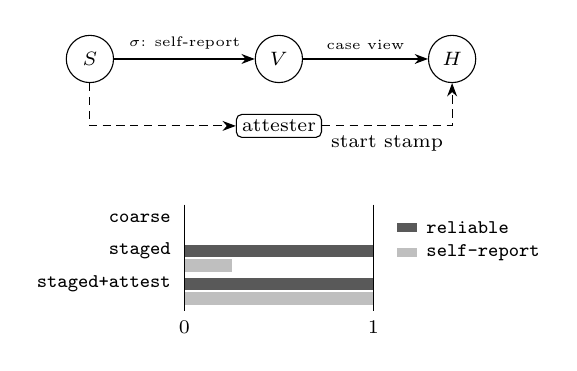
\begin{tikzpicture}[font=\scriptsize, >=Stealth,
  p/.style={draw, circle, minimum size=6mm, inner sep=0pt}]
\node[p] (S) at (0,0) {$S$};
\node[p] (V) at (2.4,0) {$V$};
\node[p] (H) at (4.6,0) {$H$};
\draw[->] (S) -- node[above, font=\tiny]{$\sigma$: self-report} (V);
\draw[->] (V) -- node[above, font=\tiny]{case view} (H);
\node[draw, rounded corners=2pt, inner sep=2pt] (A) at (2.4,-0.85) {attester};
\draw[->, densely dashed] (S) |- (A);
\draw[->, densely dashed] (A) -| node[pos=0.25, below]{start stamp} (H);
\begin{scope}[shift={(0.2,-1.9)}]
\foreach \i/\m/\r/\s in {0/coarse/0/0, 1/staged/1/0.25, 2/staged+attest/1/1}{
  \node[anchor=east] at (0.95,-\i*0.42-0.12) {\texttt{\m}};
  \fill[black!65] (1,-\i*0.42-0.2) rectangle ++(\r*2.4,0.16);
  \fill[black!25] (1,-\i*0.42-0.38) rectangle ++(\s*2.4,0.16);
}
\draw (1,0.05) -- (1,-1.3);
\draw (3.4,0.05) -- (3.4,-1.3) node[below]{1};
\node[below] at (1,-1.3) {0};
\fill[black!65] (3.7,-0.3) rectangle ++(0.25,0.12); \node[anchor=west] at (3.95,-0.24) {\texttt{reliable}};
\fill[black!25] (3.7,-0.62) rectangle ++(0.25,0.12); \node[anchor=west] at (3.95,-0.56) {\texttt{self-report}};
\end{scope}
\end{tikzpicture}
\caption{P2 in the composition family. $H$ observes $S$ only through $V$'s relay of $S$'s self-report $\sigma$, unless an attester stamps $S$'s start. Bars: determinable mass of $H$'s stage dependency under each observation model, with honest reporting (\texttt{reliable}) and with premature reports admitted (\texttt{self-report}).}
\label{fig:p2}
\end{figure}

\begin{table}[t]
\centering
\caption{P2: determinable mass of the composition's dependencies under three observation models of $V$'s case. Amb.: ambiguous observation classes.}
\label{tab:p2}
\footnotesize
\setlength{\tabcolsep}{3pt}
\begin{tabular}{@{}llccc@{}}
\toprule
Profile & Model & Amb. & \texttt{temporal} & \texttt{delivery} \\
\midrule
\tabinput{tables/p2}
\bottomrule
\end{tabular}
\end{table}

\paragraph{P3} \Cref{tab:p3} compares \arm{Hybrid} with each variant: world--dependency pairs where the variant makes a false claim the hybrid does not (safety lost) and where an outcome determined for the hybrid is not determined for the variant (observation lost). The ablation loses safety in every family and observation only in \family{reservation}, the one family where it also changes conduct.

\begin{table}[t]
\centering
\caption{P3: \arm{Hybrid} against each variant, summed over profiles; safety lost / observation lost.}
\label{tab:p3}
\small
\setlength{\tabcolsep}{4pt}
\begin{tabular}{@{}lcccc@{}}
\toprule
Family & \arm{Hyb-noE} & \arm{Chor} & \arm{Fsm} & \arm{Comm} \\
\midrule
\tabinput{tables/p3}
\bottomrule
\end{tabular}
\end{table}

\section{Worked Example}
\label{sec:example}

The episode of \cref{sec:intro} is one world of the \family{handoff} family under the \texttt{stale-read} profile, which admits a lost acceptance reply, a lost start notice and a read-back that is fresh, stale or unavailable. In this world, of probability $1/20$ under the profile, the provider $V$ accepts at instant 1 (before the acceptance deadline at 3) and initiates care at 5 (before the care deadline at 10). Its acceptance reply and its start notice are both dropped. The independent attester's confirmation of care initiation is delivered at 7. The hospital's read of $V$'s record at 11 is served as of instant 0. Both dependencies hold: $\truth(w, \texttt{flow}) = \truth(w, \texttt{temporal}) = \Ful$, for every arm, since no \family{handoff} protocol feature changes conduct.

\subsection{Observations}

Each arm's participant receives what its protocol defines:
\begingroup\raggedright
\begin{itemize}
\item \arm{Chor}: \texttt{((read-ok 11 (last-message none)))}. The protocol defines a start notice, which was dropped; the session log as of instant 0 holds nothing.
\item \arm{Fsm}: \texttt{((read-ok 11 (state referred)))}.
\item \arm{Comm}: \texttt{((read-ok 11 (ledger none none)))}: neither commitment appears in the ledger as of instant 0.
\item \arm{Hybrid} and \arm{Hybrid-noE}: \texttt{((msg ATTEST 7 5) (read-ok 11 (full referred \#f \#f none none 0)))}: the attestation, and the full record with its watermark, 0.
\end{itemize}
\endgroup

\subsection{Claims and classes}

\begin{table}[t]
\centering
\caption{The worked example: claims and their classes. Both dependencies are $\Ful$ in this world.}
\label{tab:example}
\footnotesize
\setlength{\tabcolsep}{3pt}
\begin{tabular}{@{}L{17mm}L{29mm}L{29mm}@{}}
\toprule
Arm & \texttt{flow} & \texttt{temporal} \\
\midrule
\arm{Chor} & $\Vio$ \newline false & $\Ind$ \newline abstained-ok \\
\arm{Fsm} & $\Vio$ \newline false & $\Vio$ \newline false \\
\arm{Comm} & $\Vio$ \newline false & $\Ind$ \newline abstained-ok \\
\arm{Hybrid} & $\Ind$ \newline abstained-miss & $\Ful$ \newline supported \\
\arm{Hybrid-noE} & $\Vio$ \newline false & $\Ful$ \newline supported \\
\bottomrule
\end{tabular}
\end{table}

\Cref{tab:example} gives the claims. \arm{Chor}'s acceptance timer fired, since no acceptance arrived by the deadline, and the session records $V$'s failure to respond: a false violation. Care is outside its projection once the acceptance branch has failed, so it abstains on the care dependency, correctly, because its observations are shared with worlds in which $V$ never accepted. \arm{Fsm}'s own timeout fired for the same reason, and it reads $V$'s state as current: \texttt{referred} means no care. Both claims are false. \arm{Comm} holds no discharge of the acceptance commitment by its deadline and judges it violated; the care commitment never detached in what the creditor holds, so it yields no judgment.

\arm{Hybrid} holds an attestation from a party other than $V$ that care was initiated at 5: the care claim is supported. For the acceptance it has no acceptance message and a record whose watermark, 0, does not cover the acceptance deadline, so E2 forbids reading the record's silence as a refusal, and it abstains. \arm{Hybrid-noE} receives the same observations and reads the stale record as authoritative: a false violation.

\subsection{What the example shows}

Every layer of the calculus appears. The truth is the same for every arm, so every difference is epistemic. \arm{Chor}, \arm{Fsm} and \arm{Comm} receive observations shared with worlds of opposite truth (\cref{thm:p1}), and the two that claim anyway are wrong. The hybrid and its ablation receive identical observations, so the ablation's error is purely interpretive (\cref{thm:p3}, clause 1).

The hybrid's abstention on the acceptance is classed abstained-miss: within this profile's support, the acceptance is determined, because $V$ can only accept on time or not at all, and an attestation of care implies that it accepted. The inference is valid in the model and invalid in the world the protocol is designed for, where acceptances can be late. The hybrid declines it, and \cref{prop:support} says why that is correct: under the \texttt{adversarial} profile, whose support contains this world and also admits late acceptances, the acceptance is undetermined at this world, the same abstention is classed abstained-ok, and a judge that drew the inference would be unsound. Determinacy, and therefore the class abstained-miss, is always relative to the modelled environment.

\section{Implications for Protocol Design}
\label{sec:implications}

The calculus and the results support design rules that hold across the paradigms. Each is stated with the result that warrants it.

\paragraph{Compute the ceiling before writing the judge} Determinable mass is a function of a protocol's features, its interface and the environment, and is computable by enumeration before any judge exists (\cref{thm:ceiling}). A dependency whose determinable mass is below one under the environment the protocol must survive cannot be judged completely and soundly by any mechanism over that interface. The remedy is to change the interface, by adding a message, an attestation or a record field, not to refine the judge. In \family{handoff}, no judge over the single-paradigm interfaces can be sound with coverage above 0.31 under the adversarial profile; the hybrid's interface raises the ceiling to 0.56.

\paragraph{Separate reports from evidence} A message or record in which a participant asserts its own performance is a report. Treated as evidence, it is the single largest source of false completion in DMBench, across every paradigm (\cref{sec:results}). Protocols that need $\Ful$ judgments about performance should define a channel through which a party other than the performer can attest it: a receipt from the executor, a stamp from a trusted clock, an access log kept by the resource.

\paragraph{Give every record a watermark} A record's silence about an event is evidence that the event did not happen only if the record is known to be complete through the instant the event would have been recorded. Records that do not state that instant force a sound judge to abstain on every negative they could otherwise establish, as the composition family's case record shows (\cref{tab:ceiling}). A completeness watermark is cheap to define and is what makes stale and lagging reads safe to use.

\paragraph{Retain responsibility until it is accepted} Every arm that keeps the delegating party responsible until its successor accepts has no accountability gap; the arm that releases on delegation leaves a quarter of the required time unowned. Retention is a protocol feature, available to state machines through guards and to commitments through pending and reactivated commitments (\cref{ax:continuity}).

\paragraph{Make remote stages distinguishable at every relay} In a composition, an observer can determine a remote party's conduct only if every relay on its path separates the truth-relevant states (\cref{thm:p2}). Forwarding a remote party's self-report does not do so when the report can be premature; an independent attestation of the remote stage does.

\paragraph{Judge by asserted instants with trusted clocks, not by arrival} Deadlines are properties of when events happen, not of when news of them arrives. Arms that judge by arrival fail under transit delay; arms that judge by a party's own clock fail under skew. A protocol with temporal dependencies should carry an instant asserted by a clock both parties trust.

\paragraph{Fence what expires} A lease whose holder can outlive it violates sharing whenever the holder overruns; regranting only on release violates the requester's deadline whenever the holder fails. Fencing tokens checked by the resource make expiry safe, and they are evidence an observer can use (\cref{fig:opep}).

\paragraph{Make $\Ind$ a first-class outcome} Every sound mechanism abstains wherever its observations do not determine the outcome. A protocol whose judgment set lacks $\Ind$ forces its participants to guess there, and \cref{thm:p1} guarantees that some of the guesses are false. Reporting abstentions, and separating abstentions on undetermined outcomes from abstentions on determined ones, is what lets a designer distinguish an interface problem from a judgment problem.

\section{Limitations and Threats to Validity}
\label{sec:limitations}

\paragraph{Models, not implementations} DMBench runs executable models of protocols, not deployed implementations. The models capture each paradigm's judgment over a scenario's observations and the conduct its protocol features decide; they do not capture transport, persistence, retry machinery or performance. The framework's secondary measures (recovery latency, complexity, evidence volume, decision cost) are not reported.

\paragraph{Finite, discrete environments} Every support is finite and every instant discrete; delays, skews and orders are enumerated choices. This is what makes the metrics exact and the determinacy relation decidable by search. It also means that the results are statements about the modelled supports. Concurrency is modelled as interleaving choices where a family has concurrent independent events, not as a general interleaving semantics over all participants.

\paragraph{Determinacy is relative to the support} By \cref{prop:support}, an abstention classed abstained-miss may be (a) a guarantee by construction that the mechanism declines to claim without run evidence, as in \family{reservation}, where fencing makes both dependencies hold in every world and the hybrid's abstained-miss is 0.50 under the adversarial profile; (b) an inference valid only because the support is narrower than the paradigm assumes, as in \cref{sec:example}; or (c) a consequence of a modelled interface, as in \family{composition}, whose case record carries no watermark, so the hybrid cannot read an open case after the delivery instant as a missing delivery. Abstained-miss is therefore an upper bound on avoidable abstention, not a measure of it.

\paragraph{Profiles are per family} Each family's profiles admit the faults its scenario is about. Metrics compare arms within a family and profile. Averages across families would weight families by the number of profiles each happens to have, and none are reported.

\paragraph{Independence of authorship} The independent arms were written by agent instances of the same model family as the reference arms, from specifications the reference author wrote. The protocol met the framework's validity rule in form and found twelve reference errors, but correlated failures between similar authors~\cite{knight1986experimental} are not excluded.

\paragraph{Sensitivity to documented readings} Eight interpretive choices remain open in the specifications. Per-cell figures for single-paradigm arms move under the alternative readings; the cross-family conclusions do not, because they hold for both sets of arms.

\paragraph{Scale and statistics} The framework's initial design was 8 families $\times$ 4 arms $\times$ 5 fault profiles $\times$ 30 seeds, with paired differences and clustered bootstrap intervals. Exact expectation replaces sampling for the primary results, so the variance those procedures control does not arise here; it will when the arms run as implementations with real transports, where pilot variance and power analysis should size the experiment~\cite{kalibera2013rigorous,efron1979bootstrap}.

\paragraph{Faults not modelled} A duplicated command is modelled as a duplicated message, not as a second execution of a non-idempotent effect~\cite{helland2012idempotence}. Forged and malformed actions are not injected, which is why hypotheses H2 and H3 are untested.

\section{Research Agenda}
\label{sec:agenda}

\paragraph{A unified ontology} The framework proposes a metamodel $\mathcal{U} = \langle C, I, B, N, A, E, L \rangle$ of coordination, interaction, behavioural, normative, authority and epistemic models with linkage rules, realized as modular OWL and SHACL with PROV-O-aligned evidence~\cite{w3c2013provo}. The calculus clarifies its division of labour: an ontology can carry the vocabulary and structural conformance of messages, acts, transitions, commitments and claims, and the distinctions of \cref{ax:nonequivalence} (a message is not an act, an act is not a commitment, a record is not truth). It cannot decide determinacy or soundness, which quantify over an environment's support. A linkage rule of the form $\mathrm{Occurs}(m) \wedge \mathrm{ValidAct}(m, a) \wedge \mathrm{Authorized}(a) \Rightarrow \mathrm{Establishes}(a, c)$ belongs in an operational judge, not in an unconditional ontology implication. The open problem is a release whose competency questions are answered against DMBench's run records.

\paragraph{Protocol selection} The framework states selection as constrained optimization: $P^\ast = \arg\max_{P} U(P, d, \Omega)$ subject to safety, required compliance, evidence adequacy above a threshold $\tau_E$ and cost within a budget. \Cref{thm:ceiling} gives the evidence constraint an exact form: evidence adequacy is determinable mass, computable from a protocol's interface and an environment before any judge is written. A selection method needs utility and cost models validated on held-out scenarios; neither exists yet.

\paragraph{Unauthorized and malformed actions} Testing hypotheses H2 and H3 requires fault classes in which participants attempt transitions they are not authorized for or send messages their type forbids, and a metric for admitted violations distinct from judgment errors.

\paragraph{Continuous time and unbounded environments} Replacing enumerated delays with timed-automaton semantics~\cite{alur1994timed} would make determinacy a symbolic rather than enumerative question, and would connect the ceiling theorem with monitorability results for timed properties~\cite{bauer2011runtime,francalanza2017monitorability}.

\paragraph{Implementations under the same judge} The executable models fix what each arm should conclude; implementations of the same arms over real transports can be judged by the same evaluator, with the models as their reference, and their divergences reported as implementation failures rather than paradigm failures.

\paragraph{Human independent teams} Repeating the differential protocol with separate human teams would test whether the eight open readings are the full set and whether correlated failures between similar authors hide others.

\section{Conclusion}
\label{sec:conclusion}

Communication verification asks whether interactions conform to a specification, state-machine verification whether transitions preserve invariants, and commitment verification whether obligations are managed. Dependency--Mechanism Adequacy asks whether the dependency a protocol exists for was managed, and whether a participant can establish that it was. The paper has shown that the second question factors into conduct, observability and interpretation, and that observability has an exact ceiling: no sound judge can claim more than its observations determine, and a canonical judge claims exactly that much. Epistemic adequacy is therefore a property of what a protocol makes observable.

Built as executable semantics over eight scenario families and thirty-six fault profiles, the calculus produced exact results. No single paradigm is safe across the families. A hybrid that refuses to accept a participant's report as evidence of its own performance, and refuses to read a record's silence beyond its watermark, made no false claim under any profile, and removing exactly those refusals made it unsafe in every family. False completion followed the evidence model, not the paradigm. Composition was decidable only with independent evidence of the remote party's stage. These conclusions held for arms written independently from the specifications, and the differential check that established it corrected the reference itself.

The result most useful to a designer is the ceiling. Before writing a judge, one can compute from a protocol's interface and an environment how much of a dependency's outcome any sound judge could ever establish, and so whether a richer interface, rather than a better judge, is what the dependency needs.


\bibliographystyle{IEEEtran}
\bibliography{bibliography/references}

\appendices
\section{Proofs}
\label{app:proofs}

Throughout, $a$ is an arm, $d$ a dependency, $\Omega_\pi = (W, \mu_\pi)$ an environment with finite support $S = \supp\mu_\pi$, and $[w]_a = \{ w' \in S : w' \sim_a w \}$ the observation class of $w$. For a judge $j$, write $j(w,d)$ for its judgment about $d$ on $\obs_a(w)$, and $\mathrm{Det}_a(d) = \{ w \in S : \truth_a(\cdot, d) \text{ is constant on } [w]_a \}$, so that $\dm_\pi(a,d) = \mu_\pi(\mathrm{Det}_a(d))$.

\begin{lemma}
\label{lem:classconst}
For every judge $j$ over $a$'s observations, $j(\cdot, d)$ is constant on each observation class.
\end{lemma}

\begin{proof}
$j(w, d)$ is a function of $\obs_a(w)$, which is constant on $[w]_a$ by definition.
\end{proof}

\begin{proof}[Proof of \cref{thm:p1}]
By \cref{lem:classconst}, $j(w_1, d) = j(w_2, d) = v$. If $v = \Ind$, $j$ abstains at both. Otherwise $v \in \{\Ful, \Vio, \Pen\}$, and since $\truth_a(w_1, d) \neq \truth_a(w_2, d)$, $v$ differs from at least one of them, so $j$ makes a false definitive claim at that world.
\end{proof}

\begin{proof}[Proof of \cref{thm:ceiling}]
(1) Let $j$ be sound and let $w \in S$ with $j(w, d) \neq \Ind$. Since every judgment in a run is made after every deadline, $j(w,d) \in \{\Ful,\Vio\}$; if a model admits $\Pen$, soundness treats it as a definitive claim and the argument is unchanged. By \cref{lem:classconst}, $j(w', d) = j(w, d)$ for every $w' \in [w]_a$, and soundness gives $j(w', d) = \truth_a(w', d)$. Hence $\truth_a(\cdot, d)$ is constant on $[w]_a$, that is $w \in \mathrm{Det}_a(d)$. So $\{ w \in S : j(w,d) \neq \Ind \} \subseteq \mathrm{Det}_a(d)$, and $\cov_\pi(j, d) \leq \dm_\pi(a,d)$ by monotonicity of $\mu_\pi$.

(2) Define $j^\star_a$ on a delivery sequence $x$ in the image $\obs_a(S)$ by: if $\truth_a(\cdot, d)$ takes a single value $v$ on $\obs_a^{-1}(x) \cap S$, return $v$; otherwise return $\Ind$; outside the image return $\Ind$. The definition depends only on $x$, so $j^\star_a$ is a judge over $a$'s observations. It is definitive at $w$ exactly when $w \in \mathrm{Det}_a(d)$, and then returns $\truth_a(w,d)$; so it is sound and $\cov_\pi(j^\star_a, d) = \mu_\pi(\mathrm{Det}_a(d)) = \dm_\pi(a, d)$.
\end{proof}

\begin{proof}[Proof of \cref{cor:interface}]
If $\dm_\pi(a,d) = 1$, $j^\star_a$ is sound with coverage 1. Conversely, a sound judge with coverage 1 has $\dm_\pi(a,d) \geq 1$ by \cref{thm:ceiling}(1). For the shortfall: a sound $j$ is definitive only on $\mathrm{Det}_a(d)$, so $\dm_\pi(a,d) - \cov_\pi(j,d) = \mu_\pi\{ w \in \mathrm{Det}_a(d) : j(w,d) = \Ind \}$, which is the abstained-miss mass.
\end{proof}

\begin{proof}[Proof of \cref{prop:monotone}]
If $\obs_a = h \circ \obs_b$ then $w \sim_b w'$ implies $w \sim_a w'$, so $[w]_b \subseteq [w]_a$. A function constant on $[w]_a$ is constant on $[w]_b$; with $\truth_a = \truth_b$, $\mathrm{Det}_a(d) \subseteq \mathrm{Det}_b(d)$, and the inequality follows.
\end{proof}

\begin{proof}[Proof of \cref{prop:support}]
Let $S \subseteq S'$ be the two supports. Soundness under $\mu'$ is a condition on every $w \in S'$, hence on every $w \in S$. Observation classes under $\mu$ are the classes under $\mu'$ intersected with $S$, so a function constant on the larger class is constant on the smaller. For the failure of the converses, \cref{sec:example} exhibits a world, its observations and a dependency that is determined under \texttt{stale-read} and not under \texttt{adversarial}, whose support contains the world and admits a late acceptance with the same observations; the canonical judge $j^\star_a$ of the first support claims $\Ful$ there, is sound under the first support, and is unsound under the second.
\end{proof}

\begin{proof}[Proof of \cref{thm:p2}]
The composite is an environment whose worlds are the reachable composite states, with $H$'s observation $\obs$ and truth $t$. Compliance-decidability is $\dm = 1$, which holds if and only if every observation class is truth-constant, that is, if and only if $\obs(s) = \obs(s')$ implies $t(s) = t(s')$ for all reachable $s, s'$. For the second part, $\sigma(s) = \sigma(s')$ and $v(s) = v(s')$ give $\obs(s) = \kappa(\sigma(s), v(s)) = \kappa(\sigma(s'), v(s')) = \obs(s')$ while $t(s) \neq t(s')$, so the first part fails for every choice of $\kappa$.
\end{proof}

\begin{proof}[Proof of \cref{thm:p3}]
(1) Equal protocol features give $\truth_{a'} = \truth_a$; equal interfaces with equal protocol features give $\obs_{a'} = \obs_a$. Determinable mass depends only on $\truth$, $\obs$ and $\mu_\pi$, so it is equal; by \cref{cor:interface} epistemic adequacy then depends only on the judge. (2) is \cref{prop:monotone} with $b = a'$. (3) Existence of strict loss: take two worlds $w_1, w_2$ with $\obs_a(w_1) \neq \obs_a(w_2)$, $h(\obs_a(w_1)) = h(\obs_a(w_2))$ and different truth; both are determined for $a$ if their classes are otherwise truth-constant, and neither is determined for $a'$. \Cref{tab:p2} gives instances, from the staged to the coarse model of the composition. (4) Changing protocol features changes the execution; in \family{reservation} the regrant-on-release rule makes \texttt{sharing} hold where expiry without fencing violates it, and expiry makes \texttt{temporal} hold where regrant-on-release violates it, so a change of protocol features can move truth in either direction. A judge that is sound for $a$ is a function of observations only, and when truth changes on a fixed observation class its definitive claims can become false; the reservation ablation's safety loss in \cref{tab:p3} is an instance.
\end{proof}

\section{Family Specifications}
\label{app:families}

Each family's success conditions are evaluated at an evaluation instant after every deadline. Constants are instants on one global time line unless a family admits clock skew. \Cref{tab:profiles} lists each family's profiles with the number of canonical worlds in each support.

\paragraph{\family{handoff}} $V$ accepts at 1 (on time), at 4 (late) or never; acceptance deadline 3. An accepted $V$ may initiate care at 5, may crash after accepting, or may report a start prematurely. The acceptance reply may be delivered, dropped or duplicated, with transit 1 or 4. The start notice (arrives 6) and the attestation (arrives 7) may be dropped. The read at 11 is fresh, stale (as of 0) or fails; under record lag the reported start is never recorded and the watermark is 3. Views: last message, state, ledger of the acceptance and care commitments, and a full view with watermark. \texttt{flow}: accepted by 3. \texttt{temporal}: care initiated by 10.

\paragraph{\family{reservation}} Grant to $h_1$ at 1 with lease until 5; $h_2$ requests at 2; deadline $D_2 = 7$. $h_1$ releases at 3, overruns to 8, or dies at 2. A release may be lost. The auditor reads $V$'s log at 11 (fresh, stale as of 4, or failed), containing the event kinds the protocol records: grants, releases and expiries from $V$, and uses and rejections from the resource's access log. Regrant rule per arm as in \cref{tab:families}; $h_2$ uses the resource for 2 once granted. \texttt{sharing}: no instant with two effective users. \texttt{temporal}: $h_2$ granted by 7.

\paragraph{\family{agreement}} $S$ accepts at 1 (arrives 2) with proposed or altered terms. $B$ confirms or rejects at 2 according to its fit-check feature. $S$ may revoke; with a revocation, $S$ processes $B$'s confirmation or its revocation first, at 3. The confirmation and the acknowledgement (arrives 4) may be lost. The read of $S$'s record at 11 is fresh, stale (as of 1) or fails. \texttt{fit}: nobody bound to altered terms. \texttt{mutual}: $B$ bound if and only if $S$ bound, with $B$'s binding decided by its binding rule.

\paragraph{\family{delegation}} $V$ accepts at 1; without capacity it delegates at 2; $S$ responds at 3. Care starts at 5 (by $V$ or $S$) or, under retention after $S$ declines, at 8; it may fail to start. DELEGATED (arrives 3), the start notice (start $+1$) and the attestation (start $+2$) may be lost. Read at 11: fresh, stale (as of 2) or failed. \texttt{continuity}: no interval between acceptance and care (or evaluation) owned by nobody. \texttt{temporal}: care by 10.

\paragraph{\family{deadline}} $V$ completes at 8, at 12 or never; deadline 10. DONE carries $V$'s stamp (true instant $\pm 3$ under skew) and arrives after transit 1 or 5. The attestation carries the true instant and arrives 2 later; it may be lost. Read at 19 of $V$'s completion record (stamp or none) may fail. \texttt{temporal}: completed by 10 in true time. \texttt{completion}: completed.

\paragraph{\family{external}} $V$ performs part A at 4 or not, dispatches part B at 5; $X$ completes B, completes it partially or does nothing at 7. DONE (arrives 6) is sent when A is done or prematurely. $X$'s receipt (arrives 8) may be lost. Read at 11: fresh, lagging (complete through 6) or failed. \texttt{internal}: A performed. \texttt{external}: B performed in full.

\paragraph{\family{composition}} $S$ commits at 2 and starts at 6, at 12, never, or declines; deadline 10. $S$ reports honestly or prematurely claims a start at 6. $V$ delivers at 14 if $S$ started and $V$ assembles. DELIVERED (arrives 15) and the attestation (start $+2$) may be lost; the read at 16 may fail. Observation models: coarse (case open or closed) and staged (case status, $S$'s reported stage and start). \texttt{temporal}: $S$ started by 10 in true time. \texttt{delivery}: $V$ delivered.

\paragraph{\family{replacement}} $V$ accepts at 1 and may withdraw at 3; $V_2$ accepts or declines at 5. Care starts at 6 (by $V$, no withdrawal), at 8 (by $V_2$) or, under retention after $V_2$ declines, at 11; deadline 10; it may fail to start. A withdrawn $V$ may emit a stale START asserting 6. Start notices and the attestation name their sender and may be lost. Registry read at 12: fresh, stale (as of 4) or failed. \texttt{continuity}: never owned by nobody. \texttt{temporal}: care by the responsible party by 10.

\begin{table*}[t]
\centering
\caption{Fault profiles and the number of canonical worlds in each support.}
\label{tab:profiles}
\small
\begin{tabular}{@{}l p{140mm} r@{}}
\toprule
Family & Profiles (support size) & Total \\
\midrule
\tabinput{tables/families}
\bottomrule
\end{tabular}
\end{table*}

\section{Adjudication Record}
\label{app:adjudication}

\Cref{tab:amend} lists the twelve causes decided against the reference arms, which were corrected. \Cref{tab:keep} lists the eight causes the specification left open; the reference reading was kept and the specification clarified.

\begin{table*}[t]
\centering
\caption{Causes decided against the reference arms (corrected in the reference).}
\label{tab:amend}
\small
\begin{tabular}{@{}l p{40mm} p{58mm} p{58mm}@{}}
\toprule
\# & Families / arms & Reference before & Corrected to \\
\midrule
A1 & seven families / \arm{Chor} & absence never evidence; never $\Vio$; asserted instants & a timed branch fires on arrival and records the partner's failure \\
A2 & \family{handoff} / \arm{Fsm} & flow $\Ful$ from state \texttt{accepted}, false on late acceptance & flow from the observer's own timeout on arrival \\
A3 & all / \arm{Hybrid-noE} & abstained where the hybrid abstains & the commitment rule applies; a successful read is authoritative over messages \\
A4 & \family{agreement} / all & a stale record read over a received acknowledgement; guessed no-read cases & the seller's binding from ACK, REVOKE or the buyer's REJECT first, then the record \\
A5 & \family{delegation}, \family{replacement} / \arm{Comm}, hybrids & abstained without an authoritative record & continuity from the commitment structure unless a record shows release or vacancy \\
A6 & \family{replacement} / \arm{Chor} & abstained on continuity & a withdrawal under release opens a vacancy until the successor accepts \\
A7 & \family{replacement} / \arm{Chor}, \arm{Comm}, hybrids & any START credited, including the stale queued one & a START counts only from the party responsible at its instant \\
A8 & \family{replacement} / \arm{Fsm}, \arm{Hybrid} & care by $V$ after withdrawal read as on time or abstained & the resume transition fires after the deadline: $\Vio$ \\
A9 & \family{external}, \family{composition}, \family{reservation} / \arm{Hybrid} & a participant's own record accepted as evidence of its performance & E1 applies to records: positive claims need an independent receipt or record \\
A10 & \family{composition} / \arm{Hybrid} & a record without watermark read as a negative & abstain; a party's own report of a late start or a refusal is an admitted negative \\
A11 & \family{reservation} / \arm{Hybrid} & abstained on stale logs & fencing tokens checked by the resource: sharing $\Ful$ unless uses overlap \\
A12 & \family{reservation} / \arm{Hybrid-noE} & $\Ful$ despite a release recorded after the successor's grant & $\Vio$ \\
\bottomrule
\end{tabular}
\end{table*}

\begin{table*}[t]
\centering
\caption{Admissible alternative readings (reference kept; residual disagreement in sequences).}
\label{tab:keep}
\small
\begin{tabular}{@{}l p{30mm} r p{55mm} p{55mm}@{}}
\toprule
\# & Family / arm & Seq. & Reference reading & Independent reading \\
\midrule
K1 & \family{agreement} / \arm{Chor} & 9 & messages checked by type, not payload: a conforming trace is fit & the acceptance's terms are in the session: confirming altered terms violates fit \\
K2 & \family{composition} / \arm{Fsm} & 3 & a closed case implies the stage completed within its guard & the coarse record holds nothing about the stage \\
K3 & \family{composition} / \arm{Comm} & 5 & the creditor rule: not seen discharged by the deadline & no ledger entry for the stage: $\Ind$ \\
K4 & \family{delegation} / \arm{Chor} & 2 & no DELEGATED and no read: $\Ind$ & no delegation in the session: $V$ held the role \\
K5 & \family{delegation} / \arm{Fsm} & 6 & the retaining guard keeps $V$ responsible in \texttt{delegated} & no cross-party obligations in an FSM: $\Ind$ \\
K6 & \family{external} / \arm{Chor}, \arm{Comm}, \arm{Hybrid-noE} & 7 & DONE reports the whole order complete & DONE is about part A only \\
K7 & \family{external} / \arm{Comm} & --- & one conjunctive commitment for both parts & one commitment per part (counted under K6) \\
K8 & \family{deadline} / \arm{Chor} & 1 & no DONE and no log: the wait timed out & completion outside the projection: $\Ind$ \\
\bottomrule
\end{tabular}
\end{table*}

\paragraph{Reproducibility} The models, the independent arms, the specifications and their dated clarifications, and every output are published with the paper. \texttt{raco test tests.rkt} runs the twenty-nine tests; \texttt{racket bench.rkt exact} reproduces \cref{app:results}; \texttt{racket bench.rkt sampled 100 results.jsonl} reproduces the sampled runs byte for byte; \texttt{racket bench.rkt propositions} reproduces \cref{tab:p1,tab:p2,tab:p3}; \texttt{racket diff.rkt} reproduces \cref{tab:diff}.

\onecolumn
\section{Complete Exact Results}
\label{app:results}

Every family, profile and arm; exact expectations over the profile's support. Columns: safety failure rate, false-completion rate, accountability gap rate, coverage, and the shares of supported, lucky, false, abstained-ok and abstained-miss claims, and of determinable claims.

{\footnotesize
\setlength{\tabcolsep}{3.2pt}
\begin{longtable}{@{}lll rrrrrrrrrr@{}}
\toprule
Family & Profile & Arm & SFR & FCR & AGR & Cov. & Sup. & Lucky & False & Ab-ok & Ab-miss & Det. \\
\midrule
\endfirsthead
\toprule
Family & Profile & Arm & SFR & FCR & AGR & Cov. & Sup. & Lucky & False & Ab-ok & Ab-miss & Det. \\
\midrule
\endhead
\bottomrule
\endfoot
\tabinput{tables/exact-full}
\end{longtable}
}


\end{document}
